% Time-stamp: <2025-02-06 16:39:31 sakaki>
\documentclass{jarticle}

\usepackage{tam}
\usepackage{fleqn}
\usepackage{bm}
\usepackage[dvipdfmx]{graphicx}
\usepackage[dvipdfmx]{color}
%\usepackage{color}
\usepackage{colordef}
\usepackage{amssymb}

%%%%%%%%%% Command alias %%%%%%%%%%
\newcommand{\IB}{$\bullet$}
\newcommand{\IC}{$\circ$}
\newcommand{\IS}{$*$}
%%%%%%%%%%%%%%%%%%%%%%%%%%%%%%%%%%%

\title{打合せメモ: 数理計画試案}
\author{富山県立大学 榊原一紀・松本卓也}
\date{}

\def\baselinestretch{1.02}
\renewcommand{\thefootnote}{\roman{footnote}}

\begin{document}
\maketitle

\section{はじめに}

図\ref{fig:tecseed}に示す電力ネットワークに対する電力クラスタの電力運
用最適化モデルを示す．
%
前回(資料2024-12-18）からの変更点として，電力変換器が出力値に応じて変換
効率が異なることを反映するために，バイナリ値をとるスイッチング変数を用意
して，区分線形な制約を用意した．

\begin{figure}[h]
 \centering
 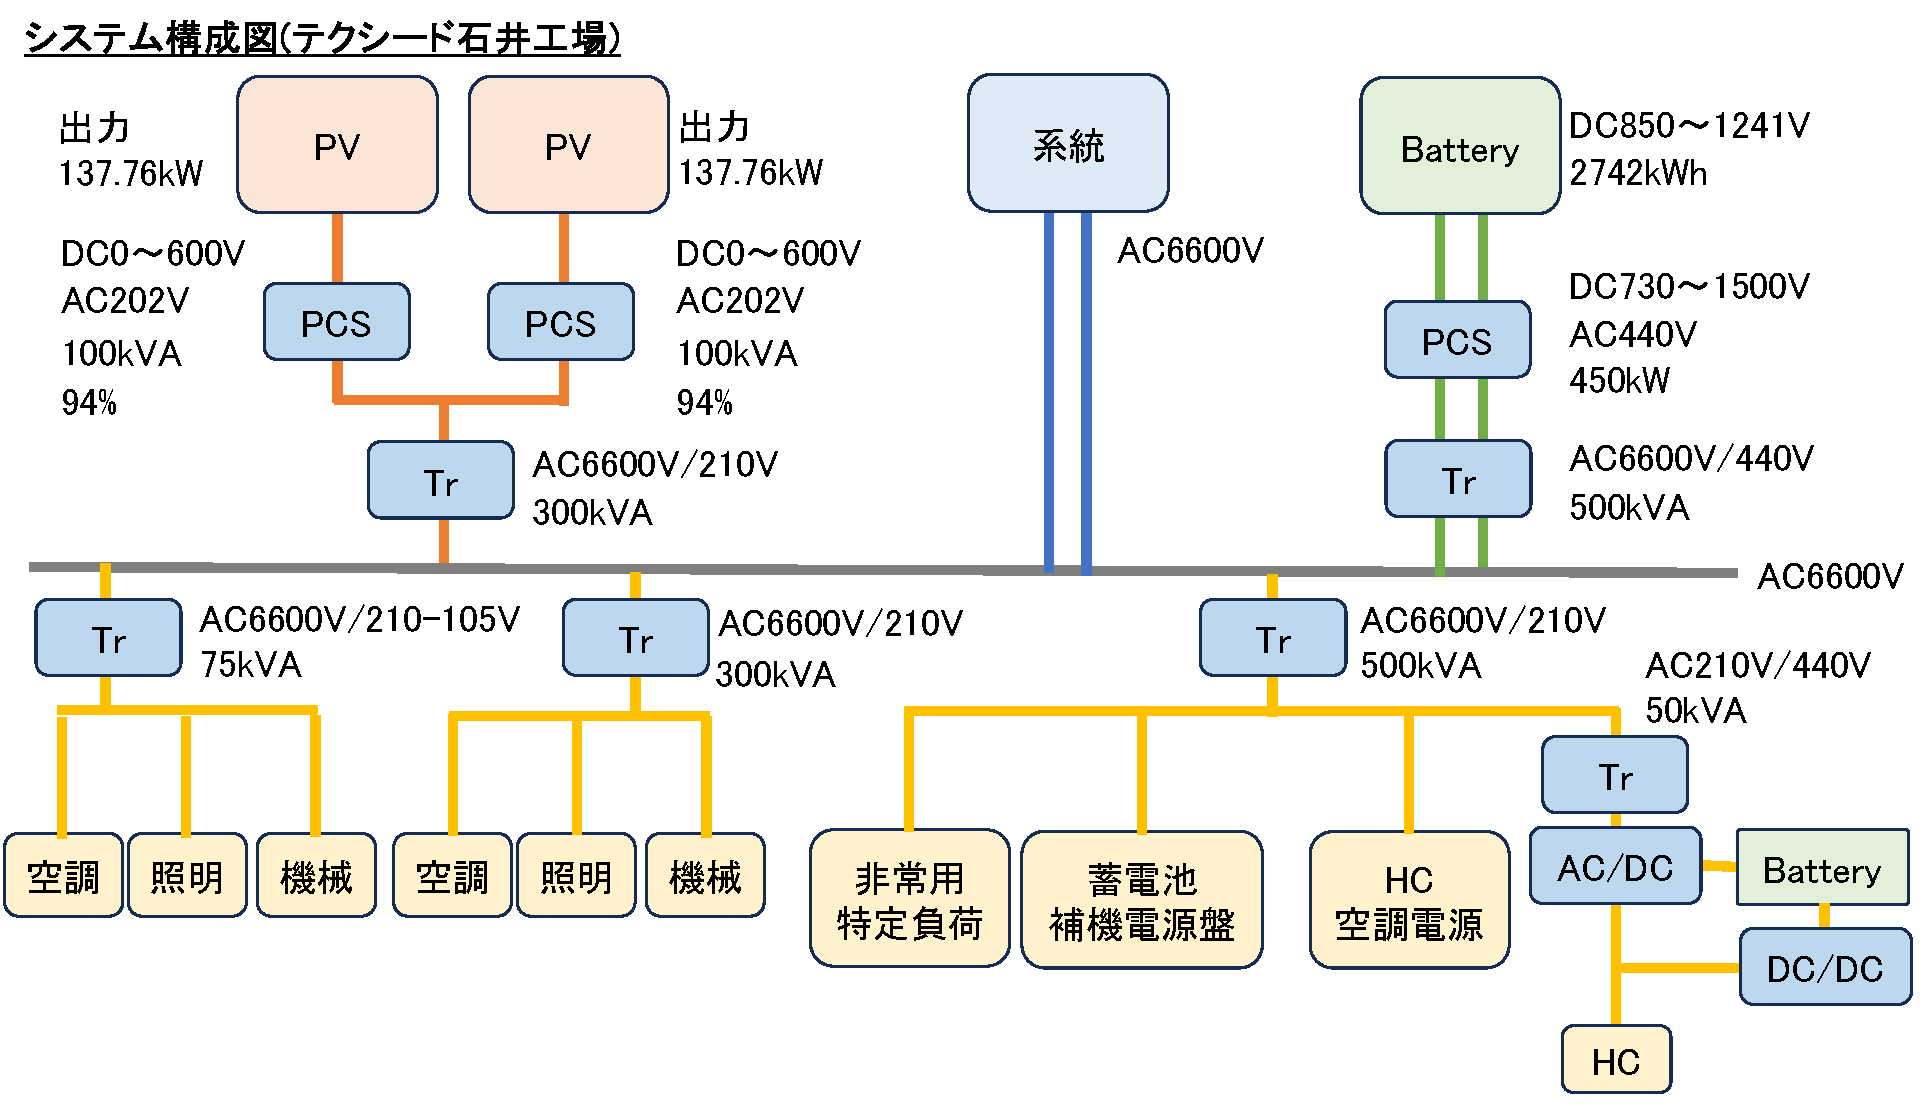
\includegraphics[width=155mm]{tecseed.pdf}
 \caption{テクシード構成図}
 \label{fig:tecseed}
\end{figure}


\section{準備}

基本要素およびそのスペックを表す定数(\IB を付して記す)と状態変数(\IC を付
して表す)として以下のものを用意する．

%\begin{itemize}
% \item[$\triangleright$] 電力クラスタC$_{i}$ $(i=1,\ldots,N)$:
\begin{itemize}
 \item[\IS] 期T$_k$ ($k=1,\ldots,K$)．各期の幅($\Delta$)は$10$秒を想定．
 \item[\IS] 太陽光発電機G
 \item[\IS] 消費機器D$^{\rm A}$
 \item[\IS] 消費機器D$^{\rm B}$
 \item[\IS] 消費機器D$^{\rm C}$
 \item[\IS] 固定バッテリーB$^{\rm F}$
  \begin{itemize}
   \item[\IB] 固定バッテリーの容量 $\overline{b}$
  \end{itemize}
 \item[\IS] 電力変換器(太陽光) E$^{\rm P}$
  \begin{itemize}
   \item[\IB] 変換効率 $\alpha^{\rm P}_{j}$, $\beta^{\rm P}_j$
              ($j=1,\ldots,J^{\rm P}$)
  \end{itemize}
 \item[\IS] 電力変換器(系統電力) E$^{\rm S}$
 \item[\IS] 電力変換器(消費機器A) E$^{\rm A}$
  \begin{itemize}
   \item[\IB] 変換効率 $\alpha^{\rm DA}_{j}$, $\beta^{\rm DA}_j$
              ($j=1,\ldots,J^{\rm DA}$)
  \end{itemize}
 \item[\IS] 電力変換器(消費機器B) E$^{\rm B}$
  \begin{itemize}
   \item[\IB] 変換効率 $\alpha^{\rm DB}_{j}$, $\beta^{\rm DB}_j$
              ($j=1,\ldots,J^{\rm DB}$)
  \end{itemize}
 \item[\IS] 電力変換器(消費機器C) E$^{\rm C}$
  \begin{itemize}
   \item[\IB] 変換効率 $\alpha^{\rm DC}_{j}$, $\beta^{\rm DC}_j$
              ($j=1,\ldots,J^{\rm DC}$)
  \end{itemize}
 \item[\IS] 電力変換器(固定バッテリー)E$^{\rm BF}$
  \begin{itemize}
   \item[\IB] 充電効率 $\alpha^{\rm FC}_{j}$, $\beta^{\rm FC}_j$
              ($j=1,\ldots,J^{\rm FC}$)
   \item[\IB] 放電効率 $\alpha^{\rm FD}_{j}$, $\beta^{\rm FD}_j$
              ($j=1,\ldots,J^{\rm FD}$)
   \item[\IB] 単位時間あたりの最大充電電量 $a^{\rm FC}$
   \item[\IB] 単位時間あたりの最大充放電量 $a^{\rm FD}$
  \end{itemize}
 \item[\IS] 系統電力S
\end{itemize}

\section{定数・変数 \mbox{\normalsize\rm 
~ (定数を「\IB」，変数を「\IC」を付して記すものとする)}}

 \begin{itemize}
  \item[\IB] 太陽光発電電力量(変換前) $g^{\rm P1}_{k}$
  \item[\IC] 太陽光発電電力量(変換後) $g^{\rm P2}_{k}$
  \item[\IC] 太陽光発電の変換効率値の採用の有無 $y^{\rm P}_{jk} \in \{1,\,0\}$
  \item[\IC] ムダ電力量 (太陽光発電出力抑制量)$v_{k}$ \\[-2.5ex]
  %
  \item[\IC] 消費電力A (変換前) $d^{\rm A1}_{k}$
  \item[\IB] 消費電力A (変換後) $d^{\rm A2}_{k}$
  \item[\IC] 消費電力Aの変換効率値の採用の有無 $y^{\rm DA}_{jk} \in \{1,\,0\}$ \\[-2.5ex]
  %
  \item[\IC] 消費電力B (変換前) $d^{\rm B1}_{k}$
  \item[\IB] 消費電力B (変換後) $d^{\rm B2}_{k}$
  \item[\IC] 消費電力Bの変換効率値の採用の有無 $y^{\rm DB}_{jk} \in \{1,\,0\}$ \\[-2.5ex]
  %
  \item[\IC] 消費電力C (変換前) $d^{\rm C1}_{k}$
  \item[\IB] 消費電力C (変換後) $d^{\rm C2}_{k}$
  \item[\IC] 消費電力Cの変換効率値の採用の有無 $y^{\rm DC}_{jk} \in \{1,\,0\}$ \\[-2.5ex]
  %
  \item[\IB] 固定バッテリーの初期SOC $b^{\rm F}_{0}$
  \item[\IC] 固定バッテリーの(期末の)SOC $b^{\rm F}_{k}$
  \item[\IC] 固定バッテリーの充電量(変換前) $x^{\rm FC1}_{k}$
  \item[\IC] 固定バッテリーの充電量(変換後) $x^{\rm FC2}_{k}$
  \item[\IC] 固定バッテリーの放電量(変換前) $x^{\rm FD1}_{k}$
  \item[\IC] 固定バッテリーの放電量(変換後) $x^{\rm FD2}_{k}$ \\[-2.5ex]
  \item[\IC] 固定バッテリーの充電効率値の採用の有無 $y^{\rm FC}_{jk} \in \{1,\,0\}$
  \item[\IC] 固定バッテリーの放電効率値の採用の有無 $y^{\rm FD}_{jk} \in \{1,\,0\}$ \\[-2.5ex]
  %
  \item[\IC] 系統電力量$s_{k}$．
  %\item[\IC] 系統電力量(変換前)$s^{1}_{k}$．
  %\item[\IC] 系統電力量(変換後)$s^{2}_{k}$．
  %\item[\IB] 変換効率$\alpha^{\rm S}$．
  %
 % \end{itemize}
\end{itemize}

\section{目的関数}

\begin{itemize}
 \item[\IS] 系統電力の最小化
 \item[\IS] 太陽光発電抑制量の最小化
\end{itemize}

\clearpage
\section{数理計画モデル}

前項で示した定数・変数を用いて，電力運用最適化問題の線形計画モデルを示す．
%
なお式中の$M$は十分大きな正の定数を表す．

\noindent
{\rm Minimize}
\begin{equation}
 \sum_{k=1}^{K} \left( s_{k} + v_{k} \right)
\end{equation}

\noindent
{\rm Subject to}
%
\begin{equation}
 g^{\rm P2}_{k} + s_{k}
 - x^{\rm FC1}_{k} + x^{\rm FD2}_{k} 
 - d^{\rm A1}_{k} - d^{\rm B1}_{k} - d^{\rm C1}_{k} - v_k = 0,
 \hfill
 k=1,\ldots,K
~~
\end{equation}
%
\begin{center} --- $ \cdot $ --- $ \cdot $ --- \end{center}
%
\begin{equation}
 g^{\rm P2}_{k} \le \alpha^{\rm P}_j g^{\rm P1}_{k} + \beta^{\rm P}_j + M\left(1-y^{\rm P}_{jk}\right),
 \hfill
 j=1,\ldots,J^{\rm P}, ~
 k=1,\ldots,K
 ~~
 \label{eq:BigM_P}
\end{equation}
%
\begin{equation}
 \sum_{j=1}^{J^{\rm P}} y^{\rm P}_{jk} = 1
 \hfill
 k=1,\ldots,K
 ~~
\end{equation}

\begin{center} --- $ \cdot $ --- $ \cdot $ --- \end{center}
%
\begin{equation}
 d^{\rm A2}_{k} \le \alpha^{\rm DA}_j d^{\rm A1}_{k} + \beta^{\rm DA}_j + M\left(1-y^{\rm DA}_{jk}\right),
 \hfill
 j=1,\ldots,J^{\rm DA}, ~
 k=1,\ldots,K
~~
 \label{eq:BigM_DA}
\end{equation}
%
\begin{equation}
 \sum_{j=1}^{J^{\rm DA}} y^{\rm DA}_{jk} = 1
 \hfill
 k=1,\ldots,K
 ~~
\end{equation}
%
\begin{equation}
 d^{\rm B2}_{k} \le \alpha^{\rm DB}_j d^{\rm B1}_{k} + \beta^{\rm DB}_j + M\left(1-y^{\rm DB}_{jk}\right),
 \hfill
 j=1,\ldots,J^{\rm DB}, ~
 k=1,\ldots,K
~~
 \label{eq:BigM_DB}
\end{equation}
%
\begin{equation}
 \sum_{j=1}^{J^{\rm DB}} y^{\rm DB}_{jk} = 1
 \hfill
 k=1,\ldots,K
 ~~
\end{equation}
%
\begin{equation}
 d^{\rm C2}_{k} \le \alpha^{\rm DC}_j d^{\rm C1}_{k} + \beta^{\rm DC}_j + M\left(1-y^{\rm DC}_{jk}\right),
 \hfill
 j=1,\ldots,J^{\rm DC}, ~
 k=1,\ldots,K
~~
 \label{eq:BigM_DC}
\end{equation}
%
\begin{equation}
 \sum_{j=1}^{J^{\rm DC}} y^{\rm DC}_{jk} = 1
 \hfill
 k=1,\ldots,K
 ~~
\end{equation}
%
\begin{center} --- $ \cdot $ --- $ \cdot $ --- \end{center}
%
\begin{equation}
 x^{\rm FC2}_{k} \le \alpha^{\rm FC}_j x^{\rm FC1}_{k} + \beta^{\rm FC}_j + M\left(1-y^{\rm FC}_{jk}\right),
 \hfill
 j=1,\ldots,J^{\rm FC}, ~
 k=1,\ldots,K
~~
 \label{eq:BigM_FC}
\end{equation}
%
\begin{equation}
 \sum_{j=1}^{J^{\rm FC}} y^{\rm FC}_{jk} = 1
 \hfill
 k=1,\ldots,K
 ~~
\end{equation}
%
\begin{equation}
 x^{\rm FD2}_{k} \le \alpha^{\rm FD}_j x^{\rm FD1}_{k} + \beta^{\rm FD}_j + M\left(1-y^{\rm FD}_{jk}\right),
 \hfill
 j=1,\ldots,J^{\rm FD}, ~
 k=1,\ldots,K
~~
 \label{eq:BigM_FD}
\end{equation}
%
\begin{equation}
 \sum_{j=1}^{J^{\rm FD}} y^{\rm FD}_{jk} = 1
 \hfill
 k=1,\ldots,K
 ~~
\end{equation}
%
\begin{equation}
 b^{\rm F}_{k} = b^{\rm F}_{k-1} + x^{\rm FC2}_{k} - x^{\rm FD1}_{k},
 \hfill
 k=1,\ldots,K
~~
\end{equation}
%
\begin{equation}
 b^{\rm F}_{k} \le \overline{b}^{\rm F},
 \hfill
 k=1,\ldots,K
~~
\end{equation}
%
\begin{equation}
 x^{\rm FC2}_{k} \le a^{\rm FC},
 \hfill
 k=1,\ldots,K
~~
\end{equation}
%
\begin{equation}
 x^{\rm FD1}_{k} \le a^{\rm FD},
 \hfill
 k=1,\ldots,K
~~
\end{equation}

\clearpage
モデル中の定数・変数と電力クラスタとの関係を図\ref{fig:structure}に示す．
%
\begin{figure}[h]
 \centering
 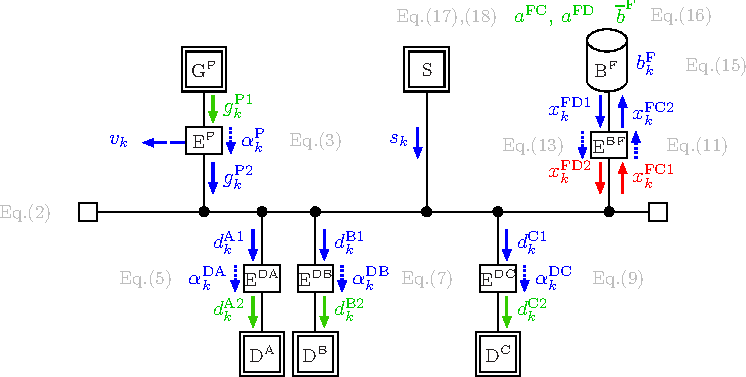
\includegraphics[width=120mm]{bus_pf.pdf}
 \caption{電力クラスタの構成図 (\textcolor{red}{赤: 決定変数}，\textcolor{blue}{青: 従属変数}，\textcolor{green3}{定数(外生変数)})}
 \label{fig:structure}
\end{figure}


\section{議論}

\begin{enumerate}
 \item 電力変換機器(E$^{\rm P}$, E$^{\rm BF}$, E$^{\rm DA}$, E$^{\rm
       DB}$およびE$^{\rm DC}$)の出力は，入力値に対してその効率値が変化す
       るものとする(つまり，入力と出力が線形の関係とならない)．さらに図
       \ref{fig:PWI}右に示すように，効率関数が下に凸な場合においては，数
       理計画として表すために，図\ref{fig:PWI}のような区分線形となる制約
       式を導入する．
       \begin{figure}[h]
        \centering
        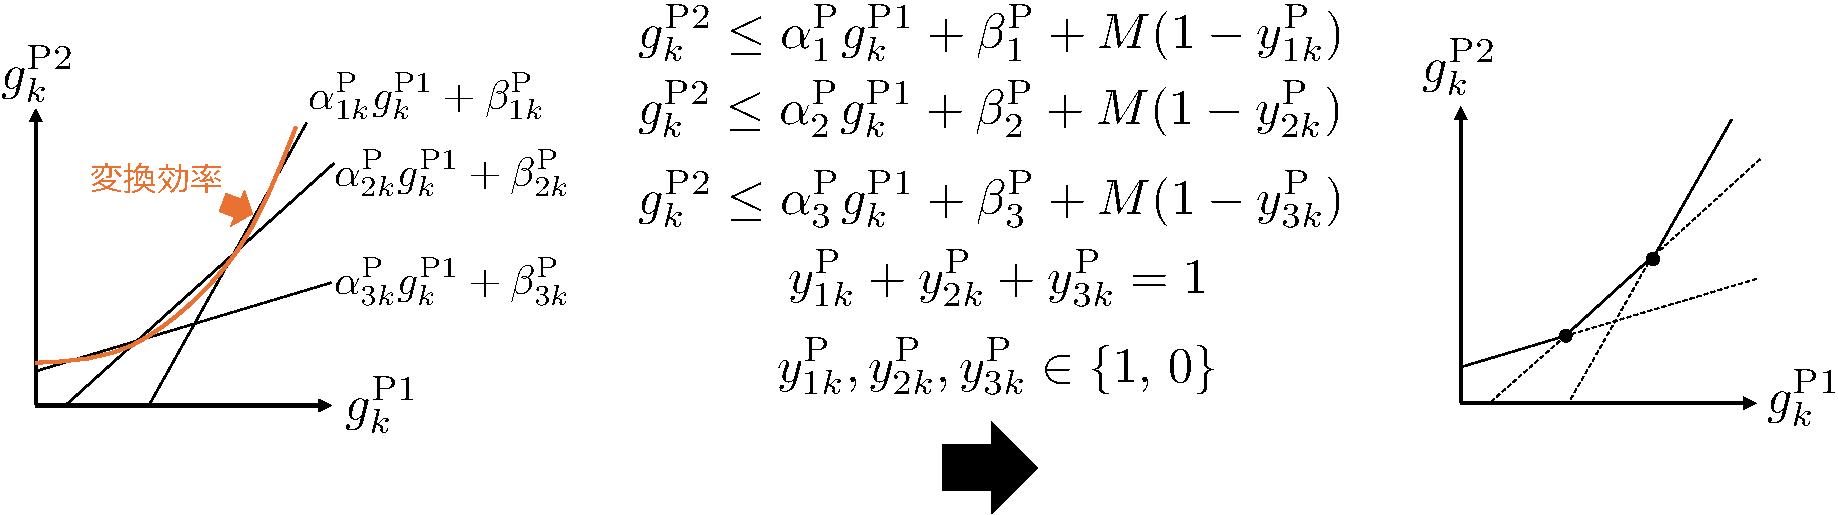
\includegraphics[width=130mm]{piecewise_linear.pdf}
        \caption{区分線形関数による表現 (太陽光発電機器の場合)}
        \label{fig:PWI}
       \end{figure}
 \item 需要電力(たとえば空調)を場合によっては出力抑制することもあり得る．
       この場合，モデル中の$d^{\rm A1}_{k}$, $d^{\rm B1}_{k}$あるいは
       $d^{\rm C1}_{k}$が変数になる?
 \item モデル中の電力機器D$^{\rm C}$は，EVの充電ステーション設備に対応し
       ている．充電ステーション内には低圧充電設備と高圧充電設備の2系統か
       ら成り，高圧充電設備にはバッテリーがある．このバッテリーの制御則
       の詳細は不明，かつこちらから操作することはできない?
\end{enumerate}

\begin{flushright}
 以上．
\end{flushright}



\section{サンプルモデル}
図\ref{fig:gP1}から図\ref{fig:dC1}に示す実績データを用いて，数理計画モデルのサンプルモデルを作成した．
各変換機の効率は一定とし，仮に0.95とした．

図\ref{fig:s_compare}に，系統買電の最適化結果と実績値の比較を示す．
また，図\ref{fig:x_compare}に，バッテリーの入出力の最適化結果と実績値の比較を示す．
系統買電実績値は，マイナスの値を持っており，逆潮流／売電を行っているのではないかと考えられる．
系統買電とバッテリーの入出力をみると，夜間の定常的な需要を，
最適化結果ではそのほとんどを系統電力から供給しているのに対して，実績ではバッテリーから供給していることがわかる．


\section{変換器効率について}
太陽光発電のPCSの入出力データから，変換効率の分析を行うため，以下のグラフを作成した．
図\ref{fig:PCS_efficiency1}は，PCSの入力電力と変換効率の関係を示したものである．
図\ref{fig:PCS_efficiency2}は，PCSの入力直流電力と出力交流電力の関係を示している．

図\ref{fig:PCS_efficiency1}から，は，PCSの入力電力が十分大きい場合には約0.95の変換効率であるが，
入力が小さいときには，変換効率が低くなる傾向があり，さらにいくつかのモードがあるように見える．
また，時間的に連続した点は同じモードに存在する傾向にあるが，ときおり別のモードにシフトしているように見える．
このように，変換効率を厳密に設定するには複雑なモデルを必要とすることが示唆される．

一方，図\ref{fig:PCS_efficiency2}からは，PCSへの入出力が，誤差はあるものの概ね線形の関係にあることがわかる．
比例関係であるともみなせると考えられる．

上記の分析や，その他の変換器のスペック・データ・知見等を前提に，さらには最適化モデルに必要とされる厳密性を考慮し，
変換効率のモデルが定数の比例係数で与えられる簡単なもので良いのか，それとも複雑なモデルが必要となるのかを検討していく必要がある．





\begin{figure}[h]
      \centering
      \begin{minipage}[b]{\linewidth}
        \centering
        
\includegraphics[width=\linewidth]{../png/gP1.png}
        \caption{太陽光発電電力実績データ}
        \label{fig:gP1}
      \end{minipage}
      \hfill
      \begin{minipage}[b]{\linewidth}
        \centering
        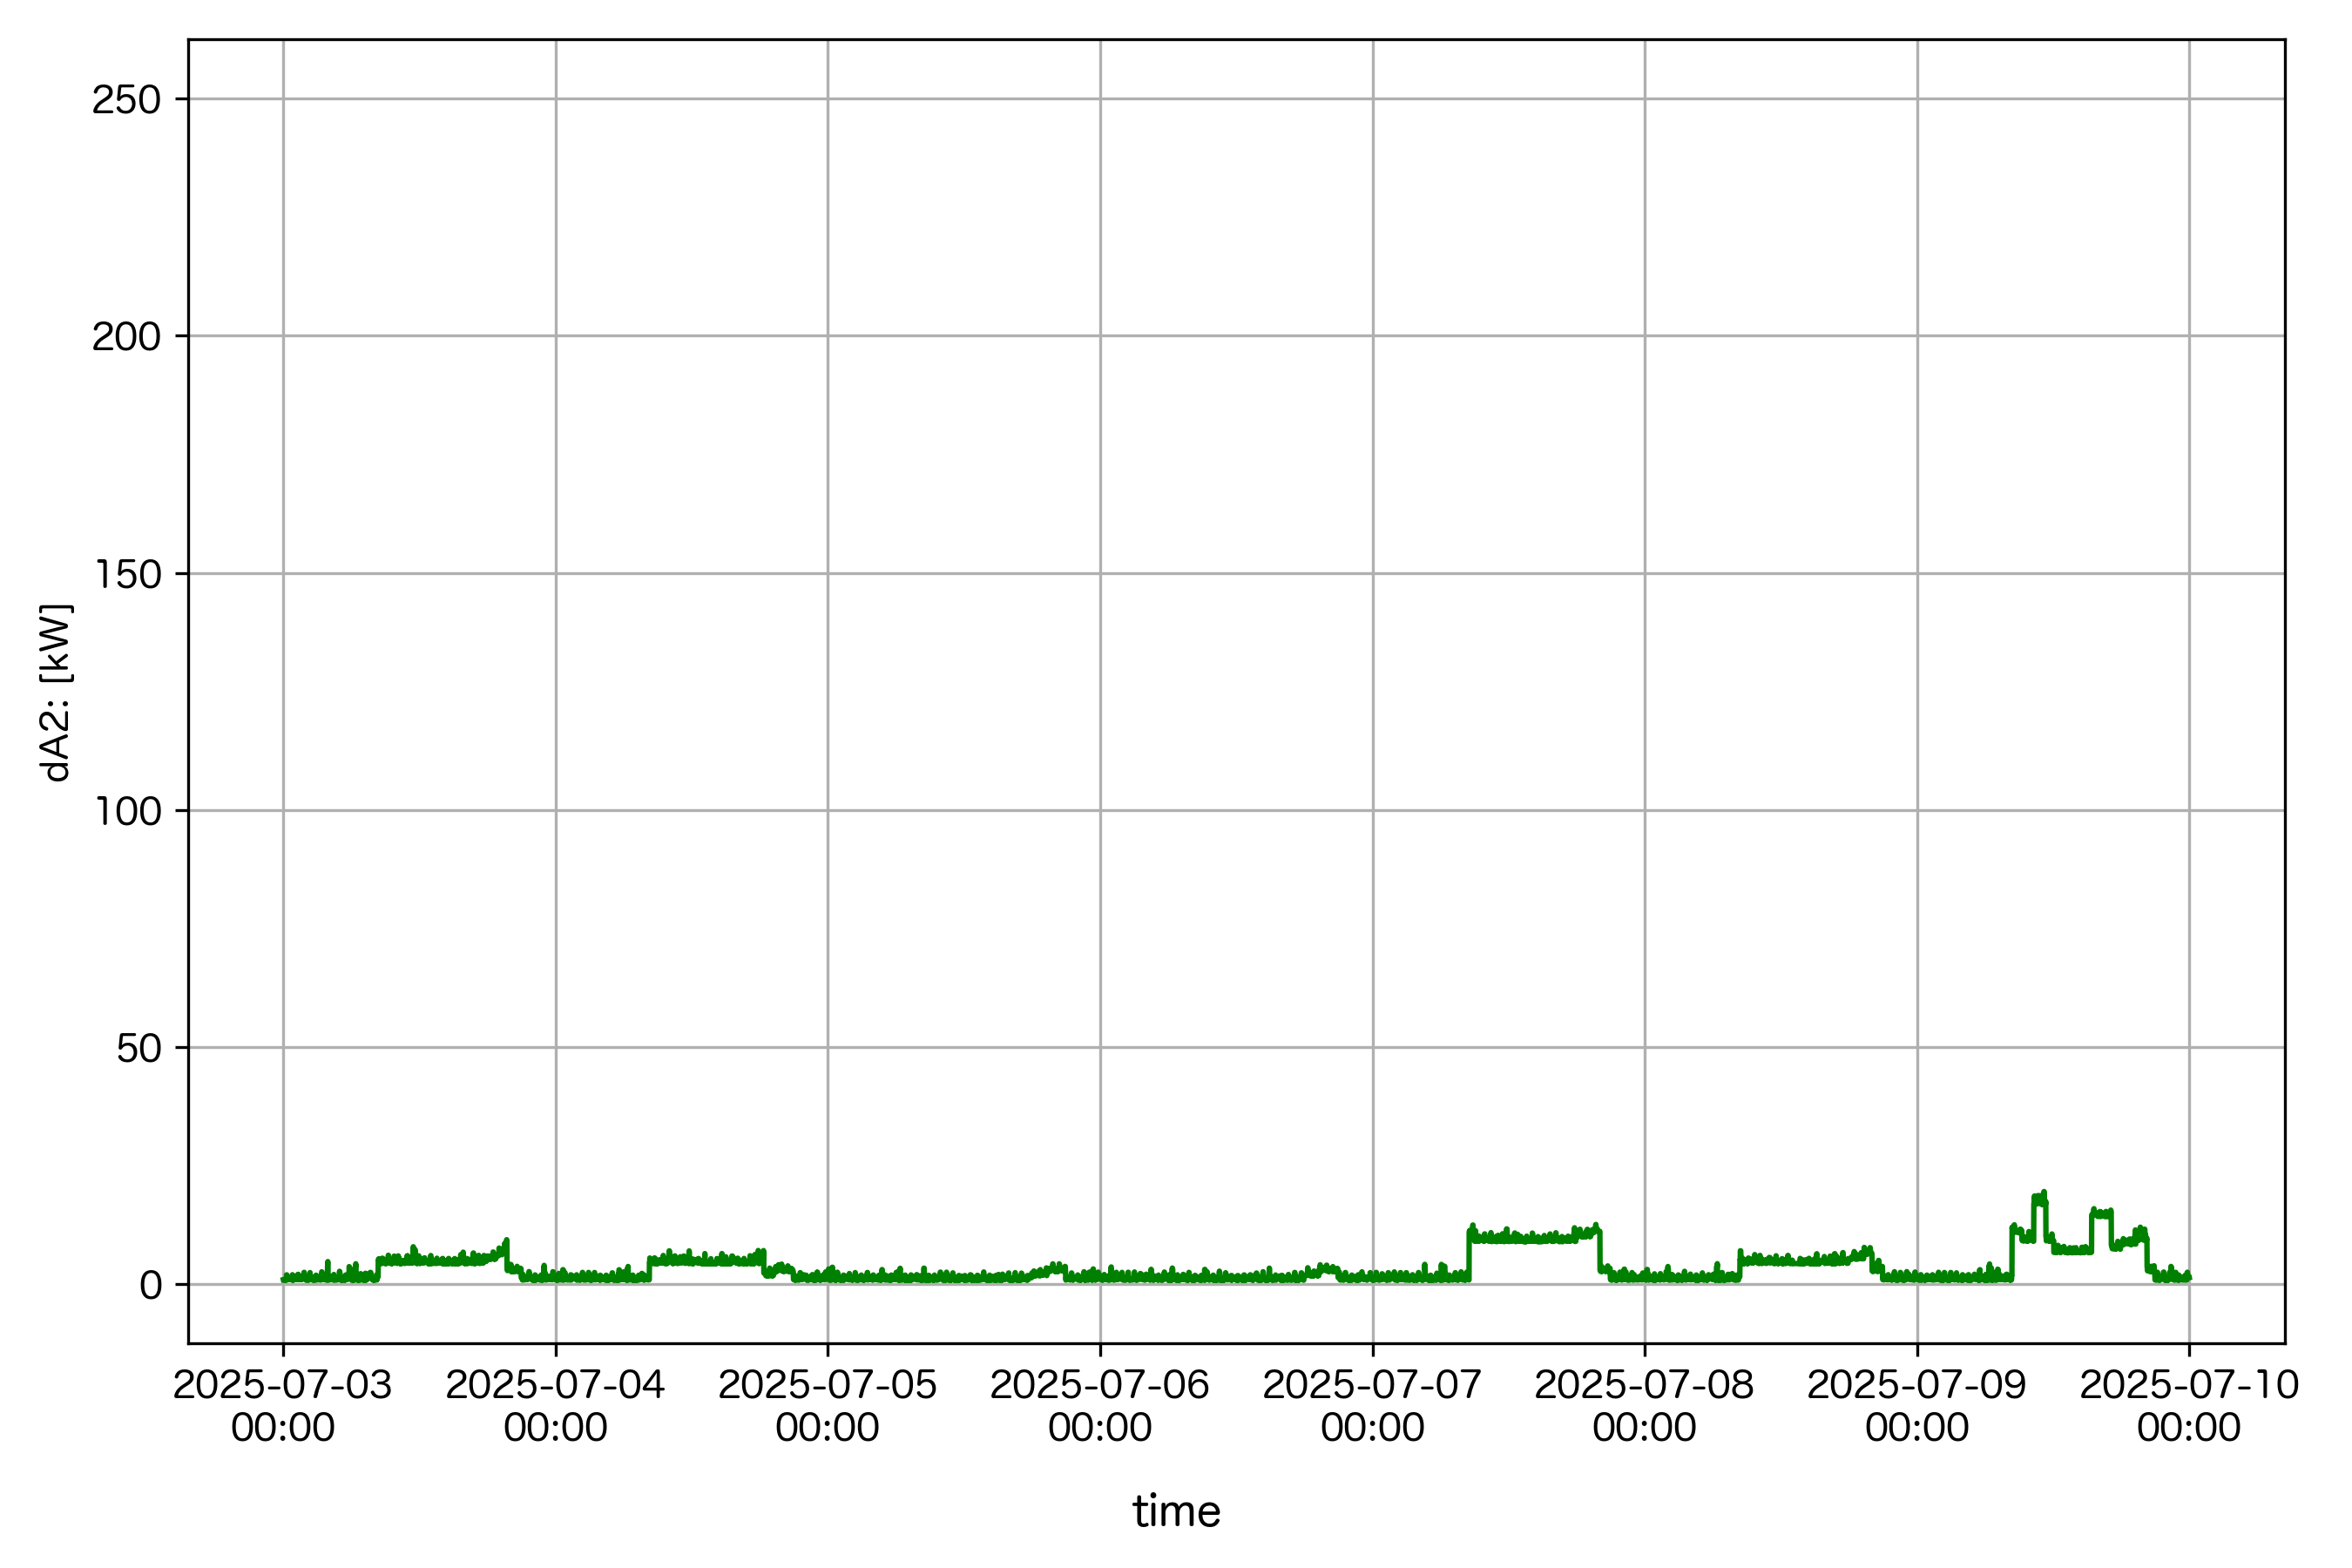
\includegraphics[width=\linewidth]{../png/dA2.png}
        \caption{消費電力A実績データ（6600/210-105V 75kVA）}
        \label{fig:dA1}
      \end{minipage}
\end{figure}


\begin{figure}[h]
      \centering
      \begin{minipage}[b]{\linewidth}
        \centering
        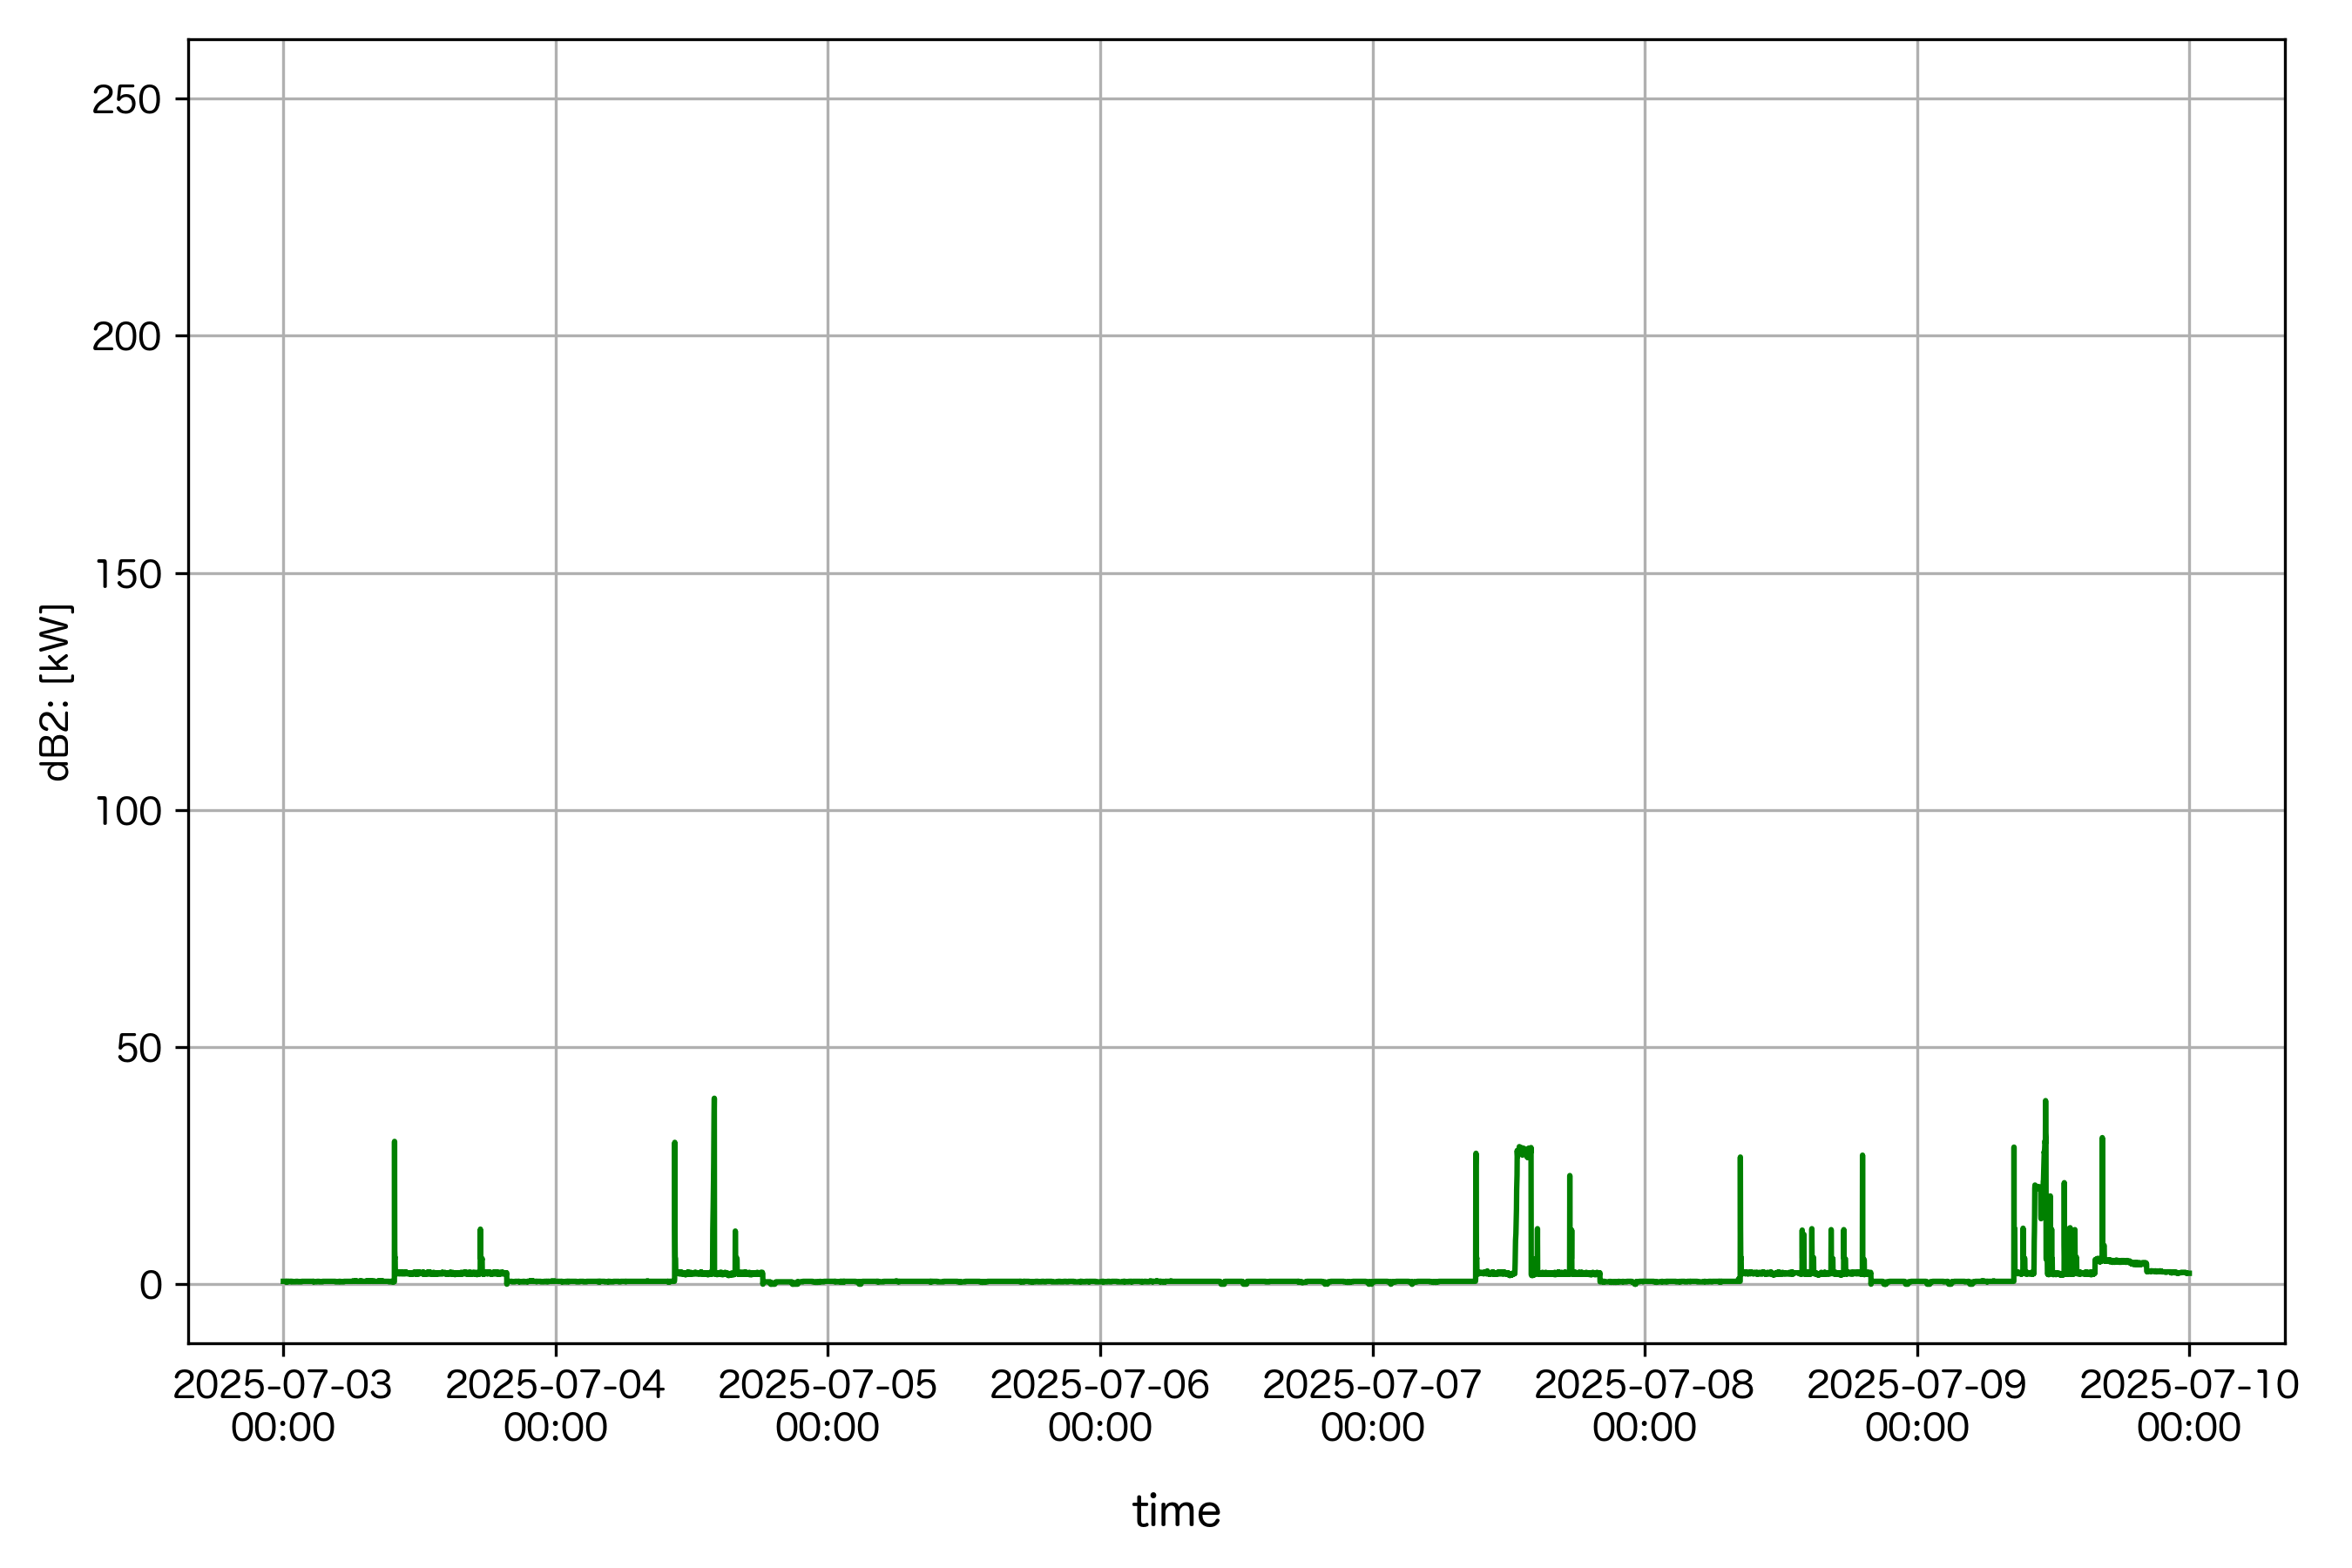
\includegraphics[width=\linewidth]{../png/dB2.png}
        \caption{消費電力B実績データ（6600/210V 300kVA）}
        \label{fig:dB1}
      \end{minipage}
      \hfill
      \begin{minipage}[b]{\linewidth}
        \centering
        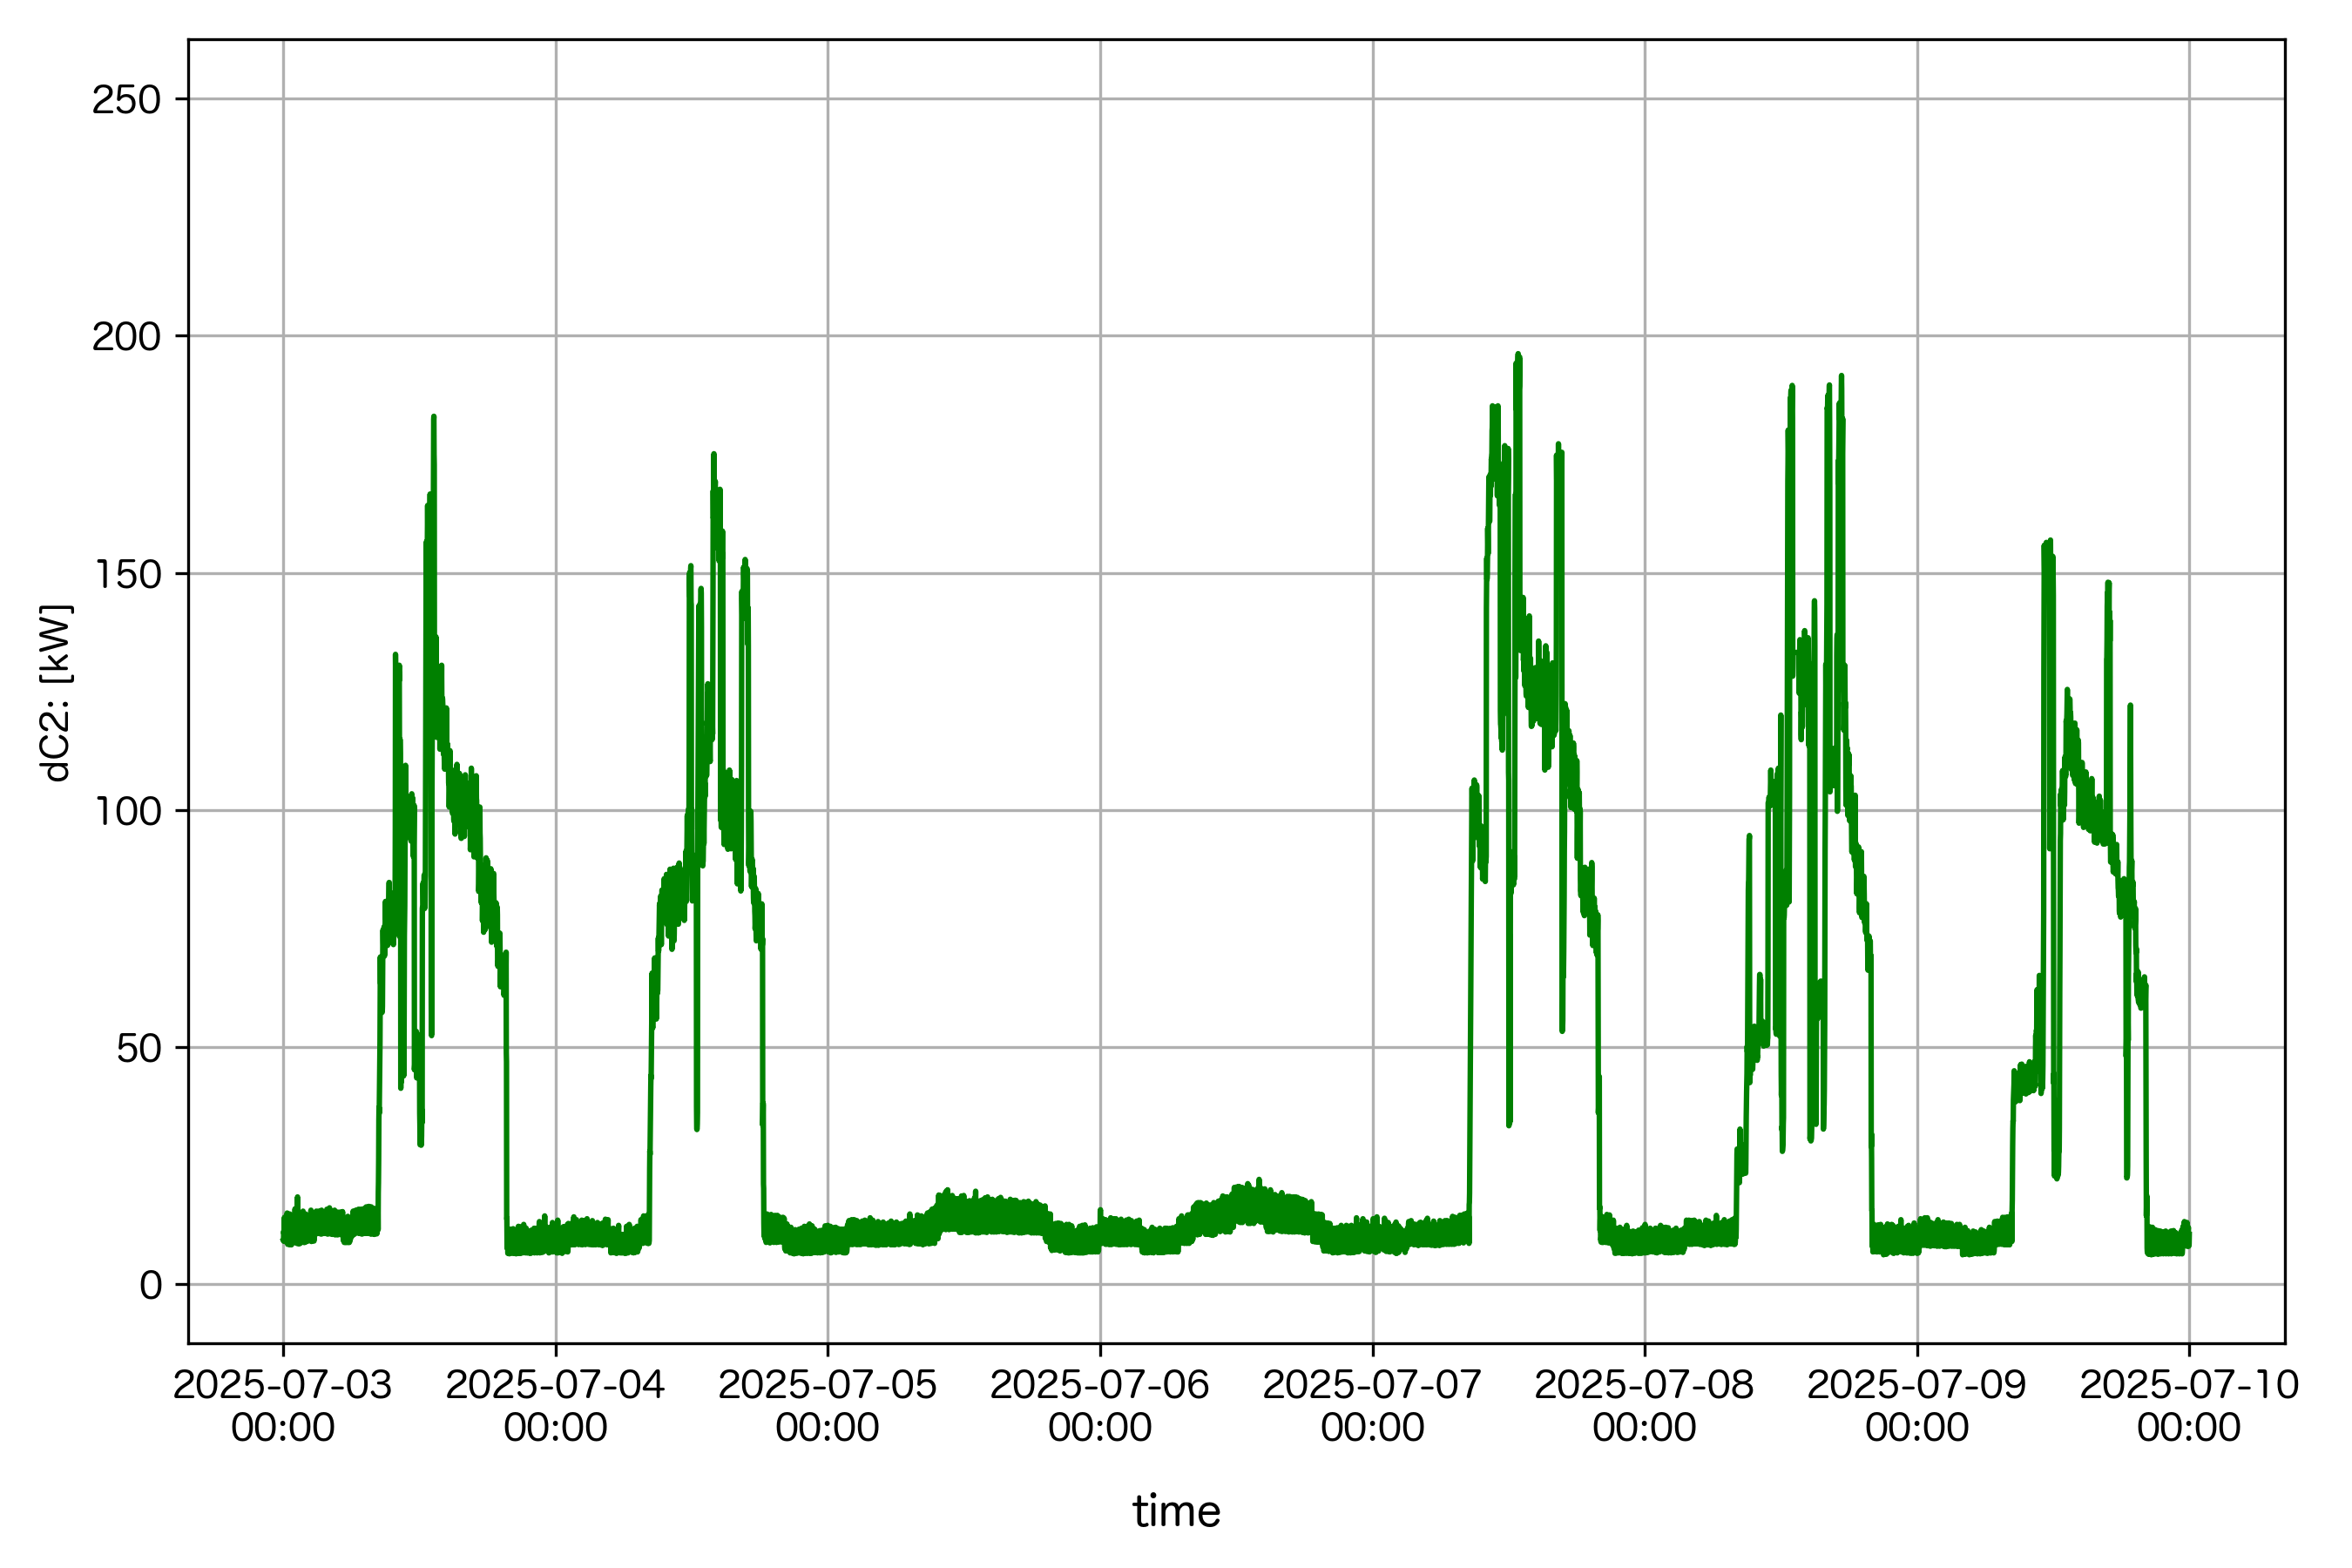
\includegraphics[width=\linewidth]{../png/dC2.png}
        \caption{消費電力C実績データ（6600/210V 500kVA）}
        \label{fig:dC1}
      \end{minipage}
\end{figure}

\begin{figure}[h]
      \centering
      \begin{minipage}[b]{\linewidth}
        \centering
        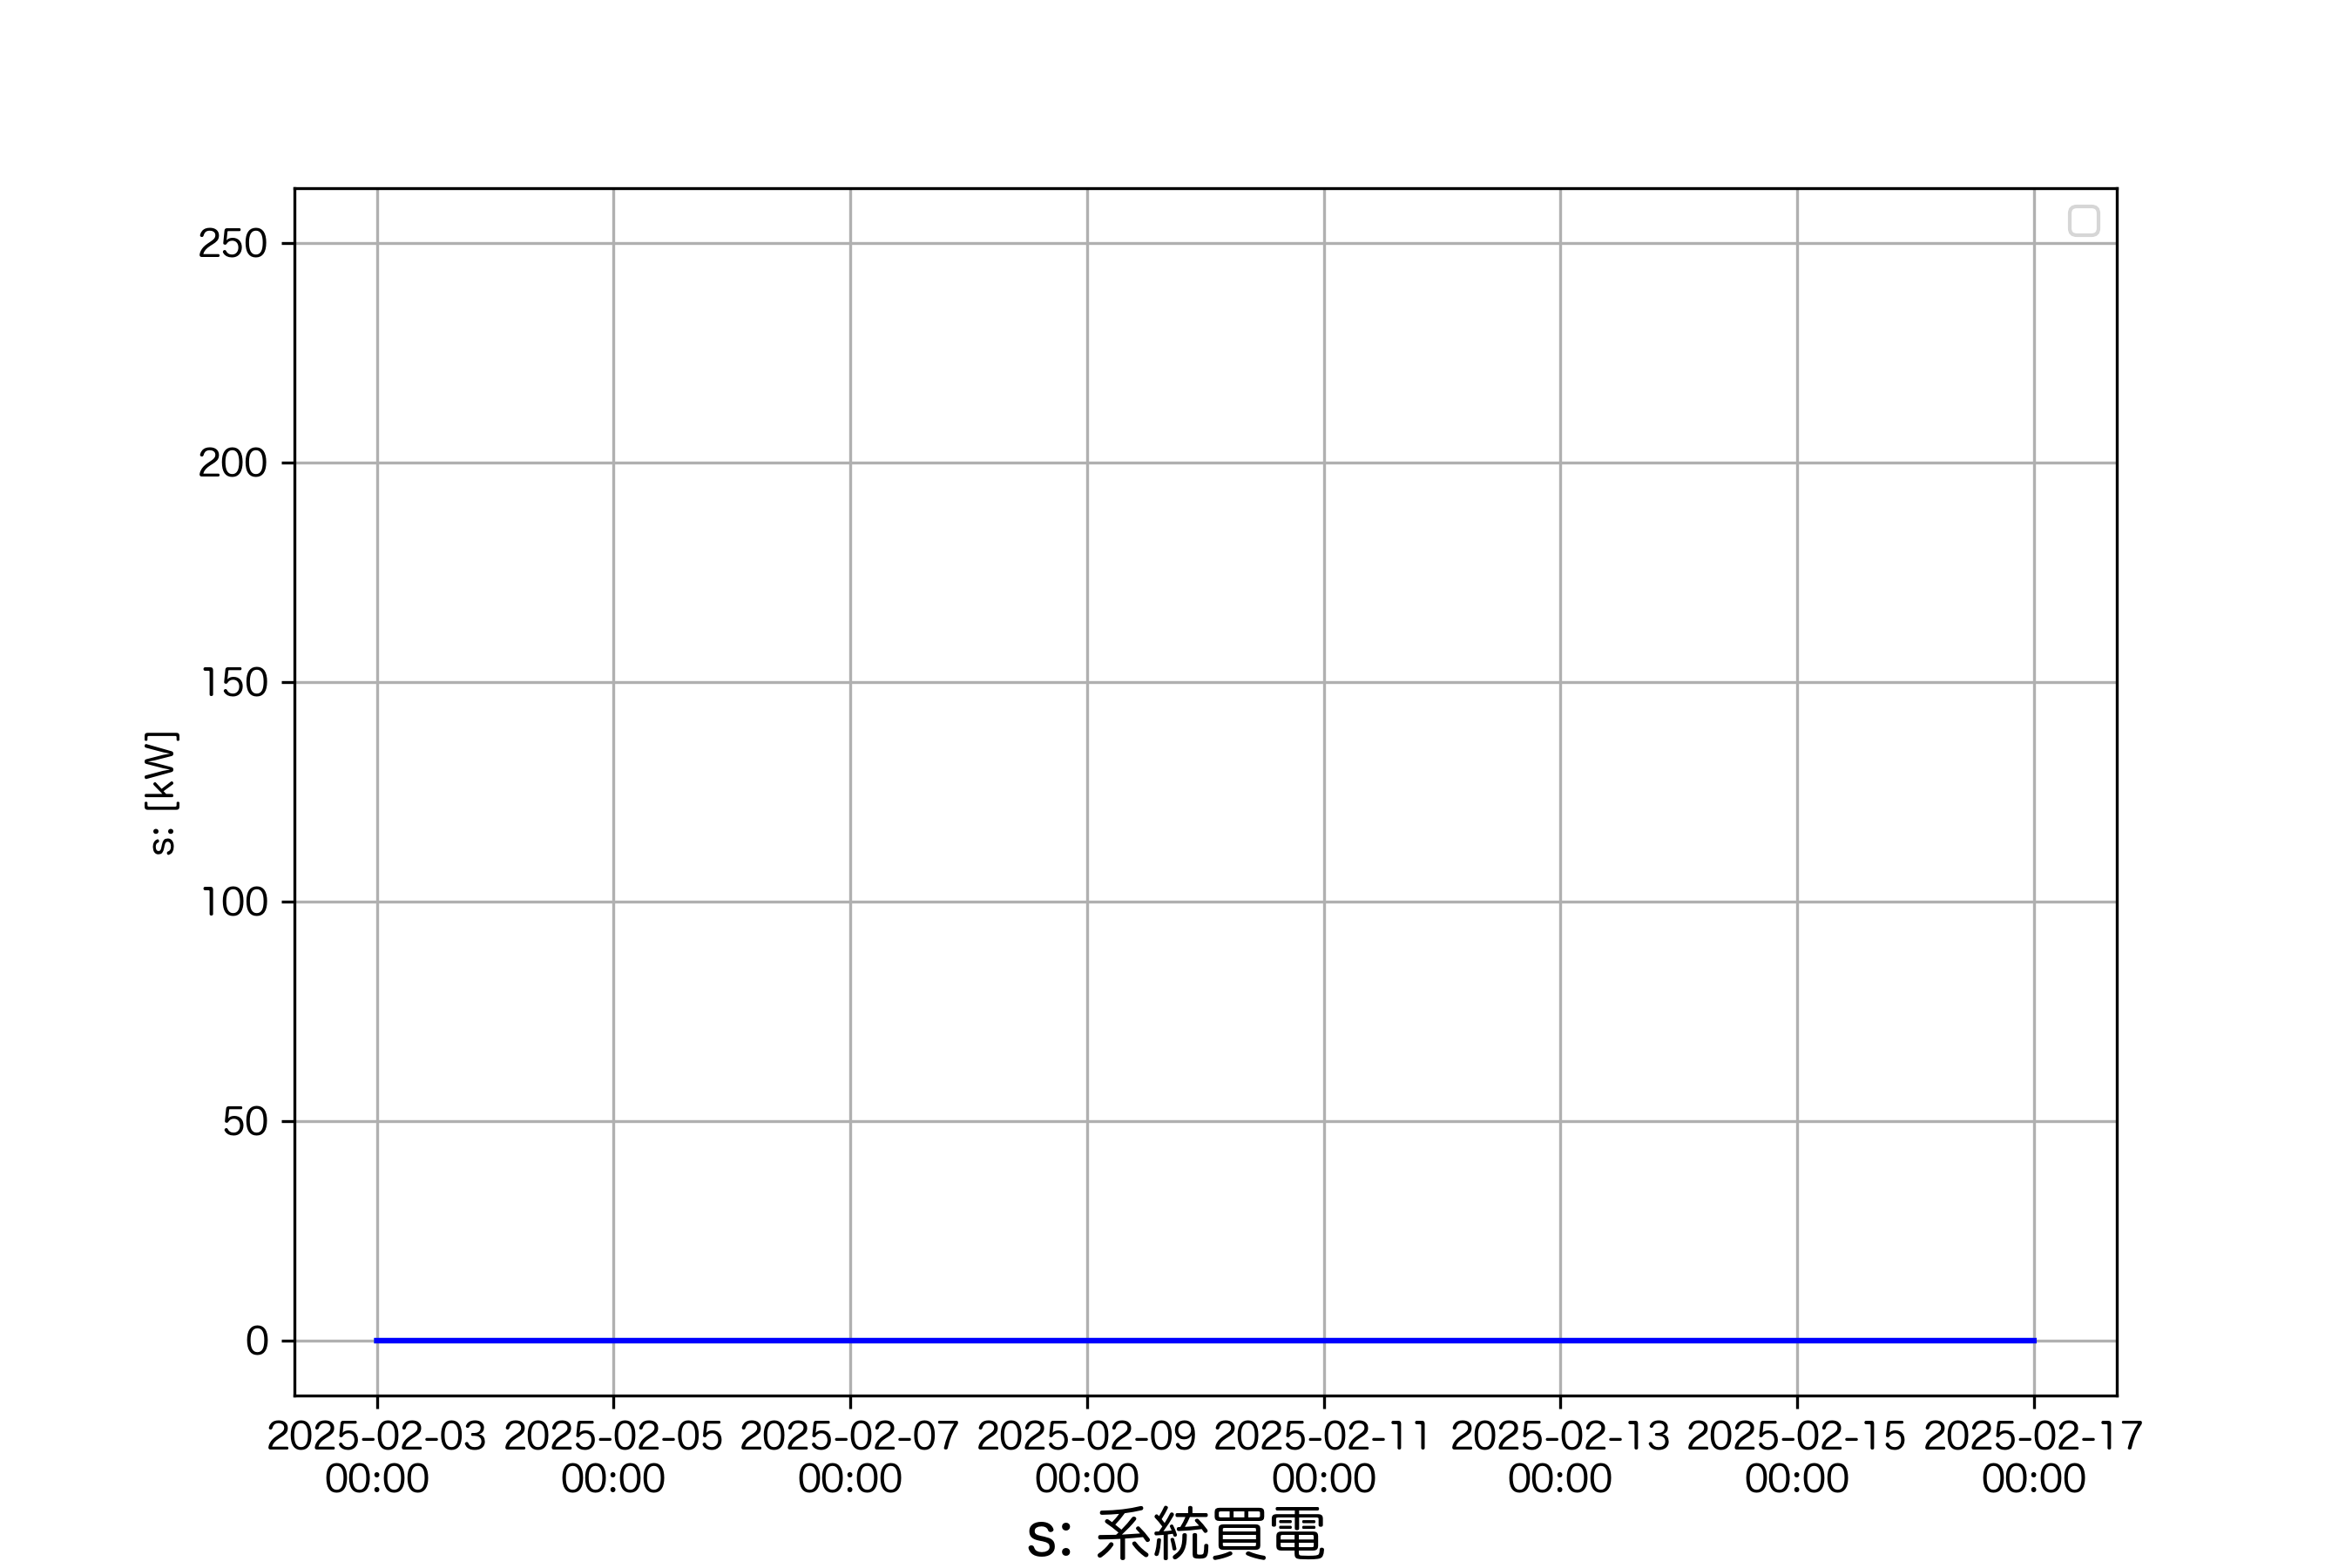
\includegraphics[width=\linewidth]{../png/s.png}
        \caption{系統買電（最適化結果）}
        \label{fig:dB1}
      \end{minipage}
      \hfill
      \begin{minipage}[b]{\linewidth}
        \centering
        
\includegraphics[width=\linewidth]{../png/bF.png}
        \caption{バッテリーSOC（最適化結果）}
        \label{fig:dC1}
      \end{minipage}
\end{figure}

\begin{figure}[h]
      \centering
      \begin{minipage}[b]{\linewidth}
        \centering
        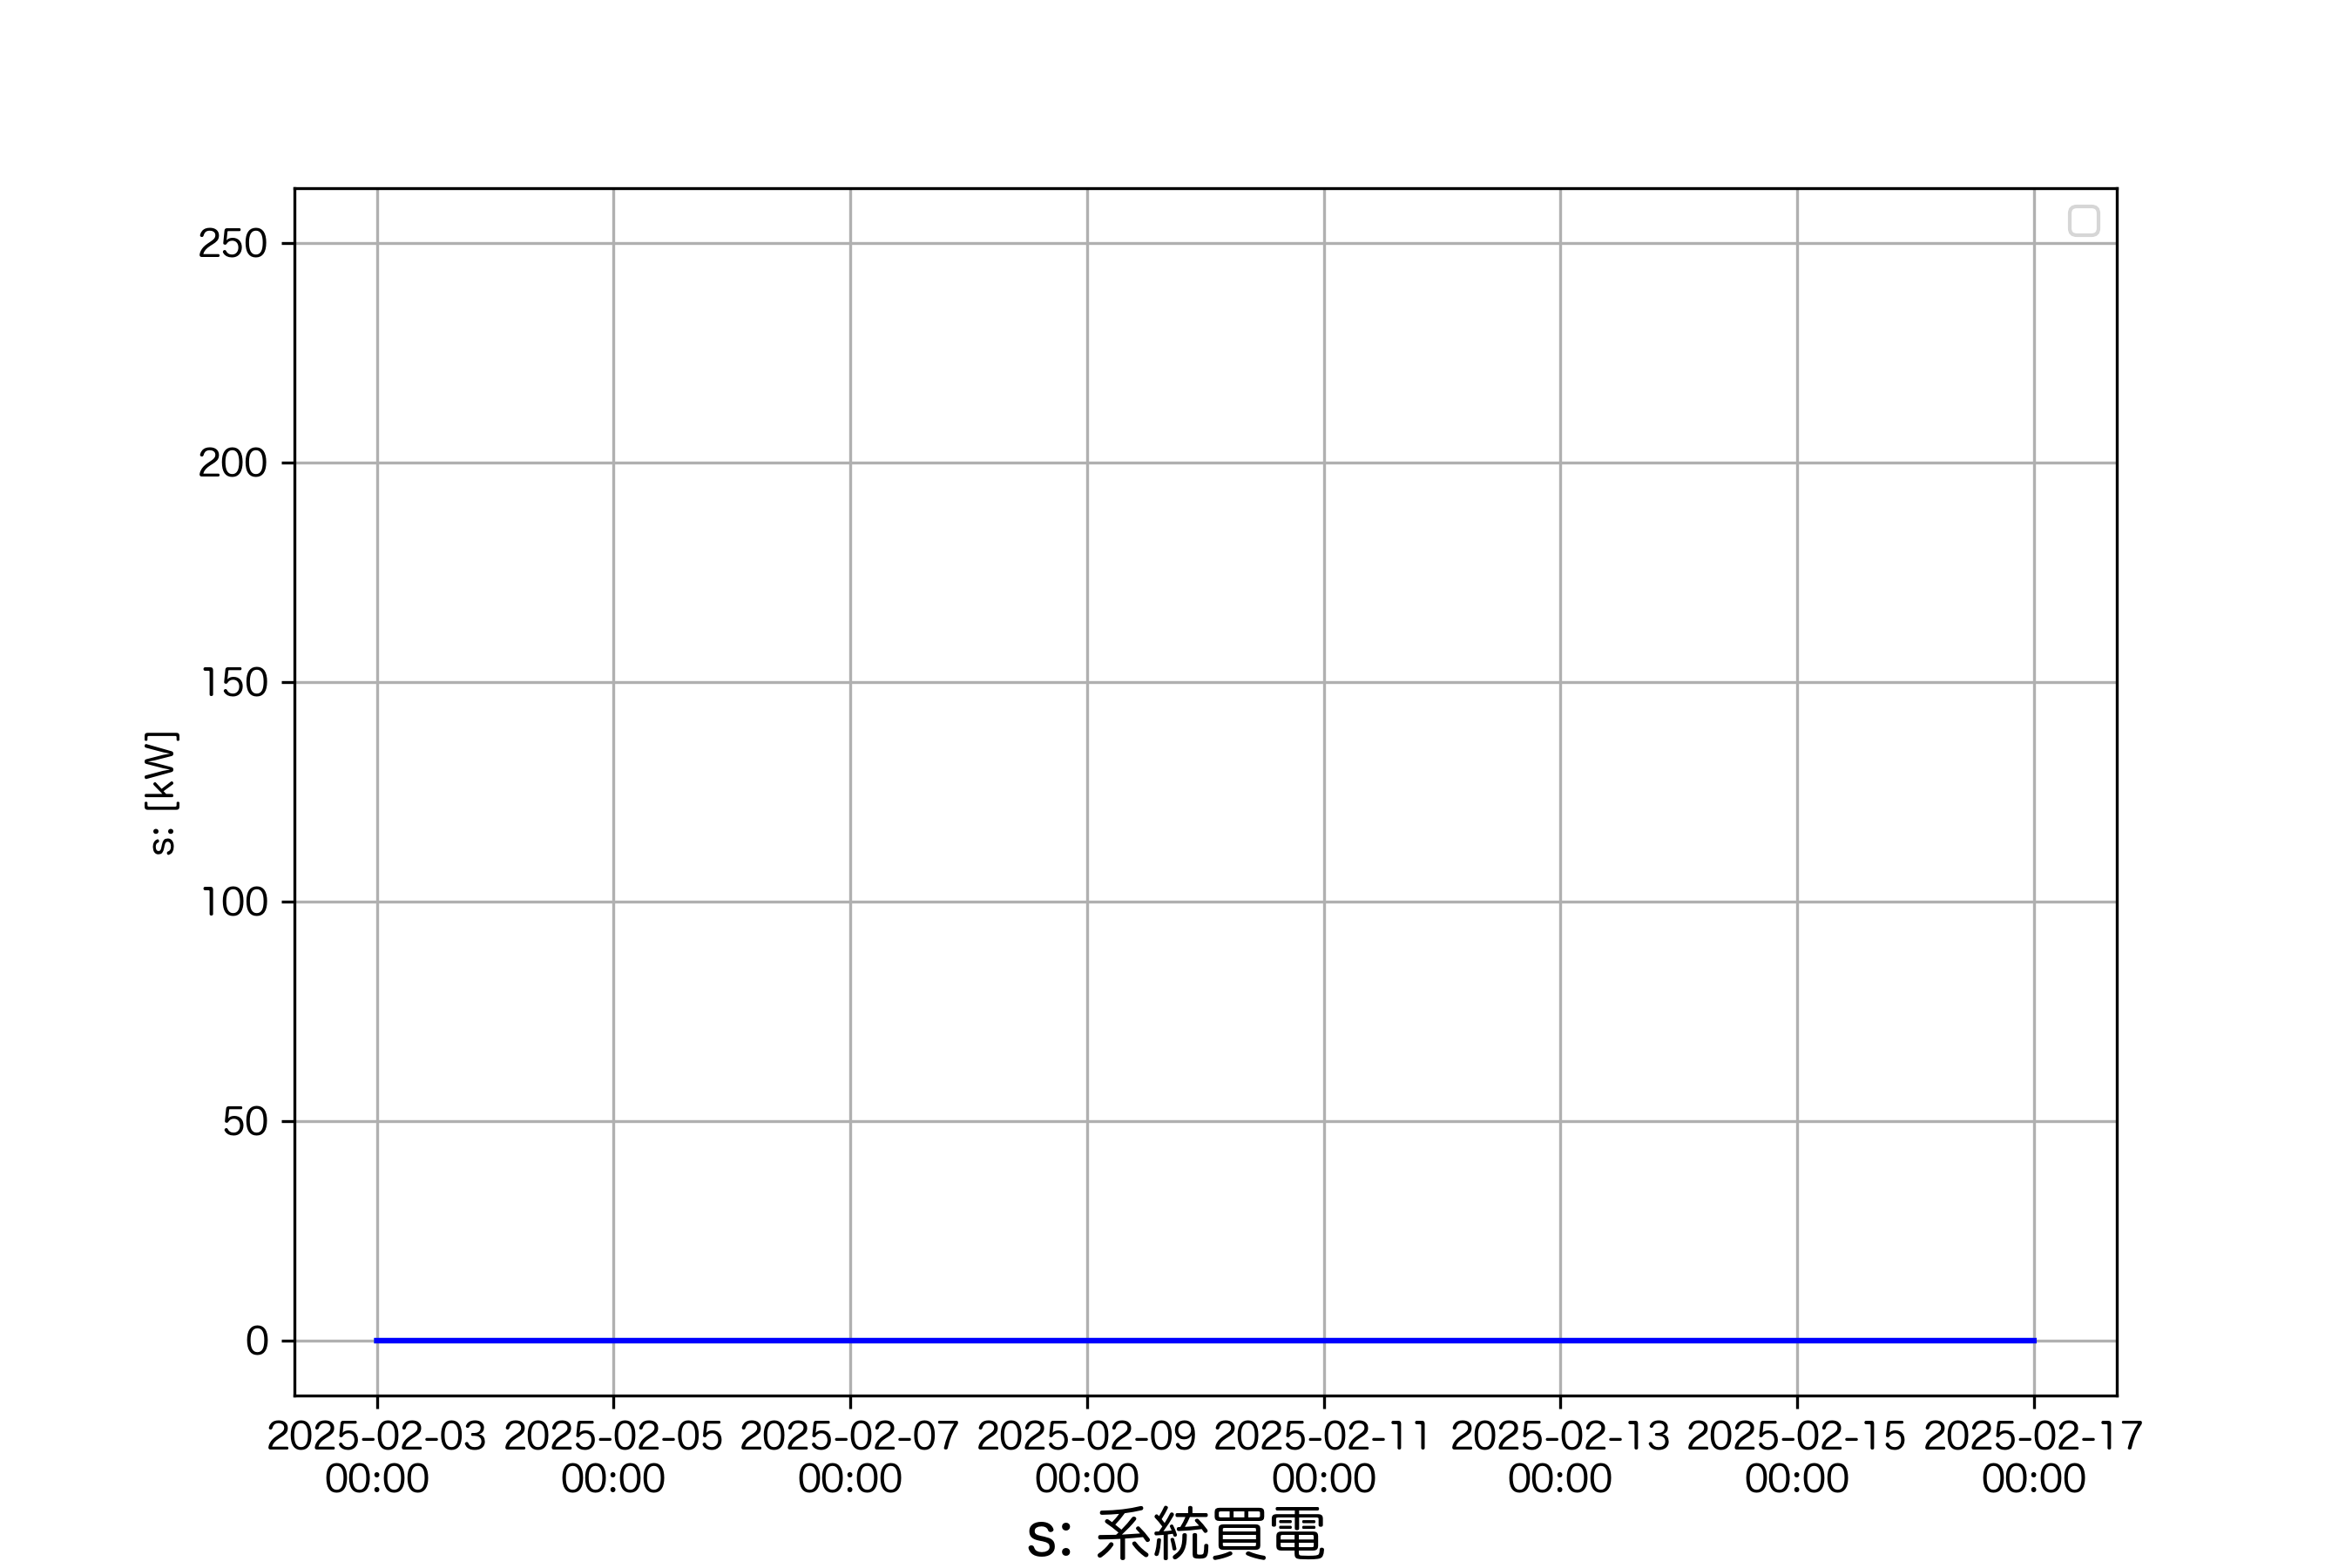
\includegraphics[width=\linewidth]{../png/s.png} 
      \end{minipage}
      \hfill
      \begin{minipage}[b]{\linewidth}
        \centering
        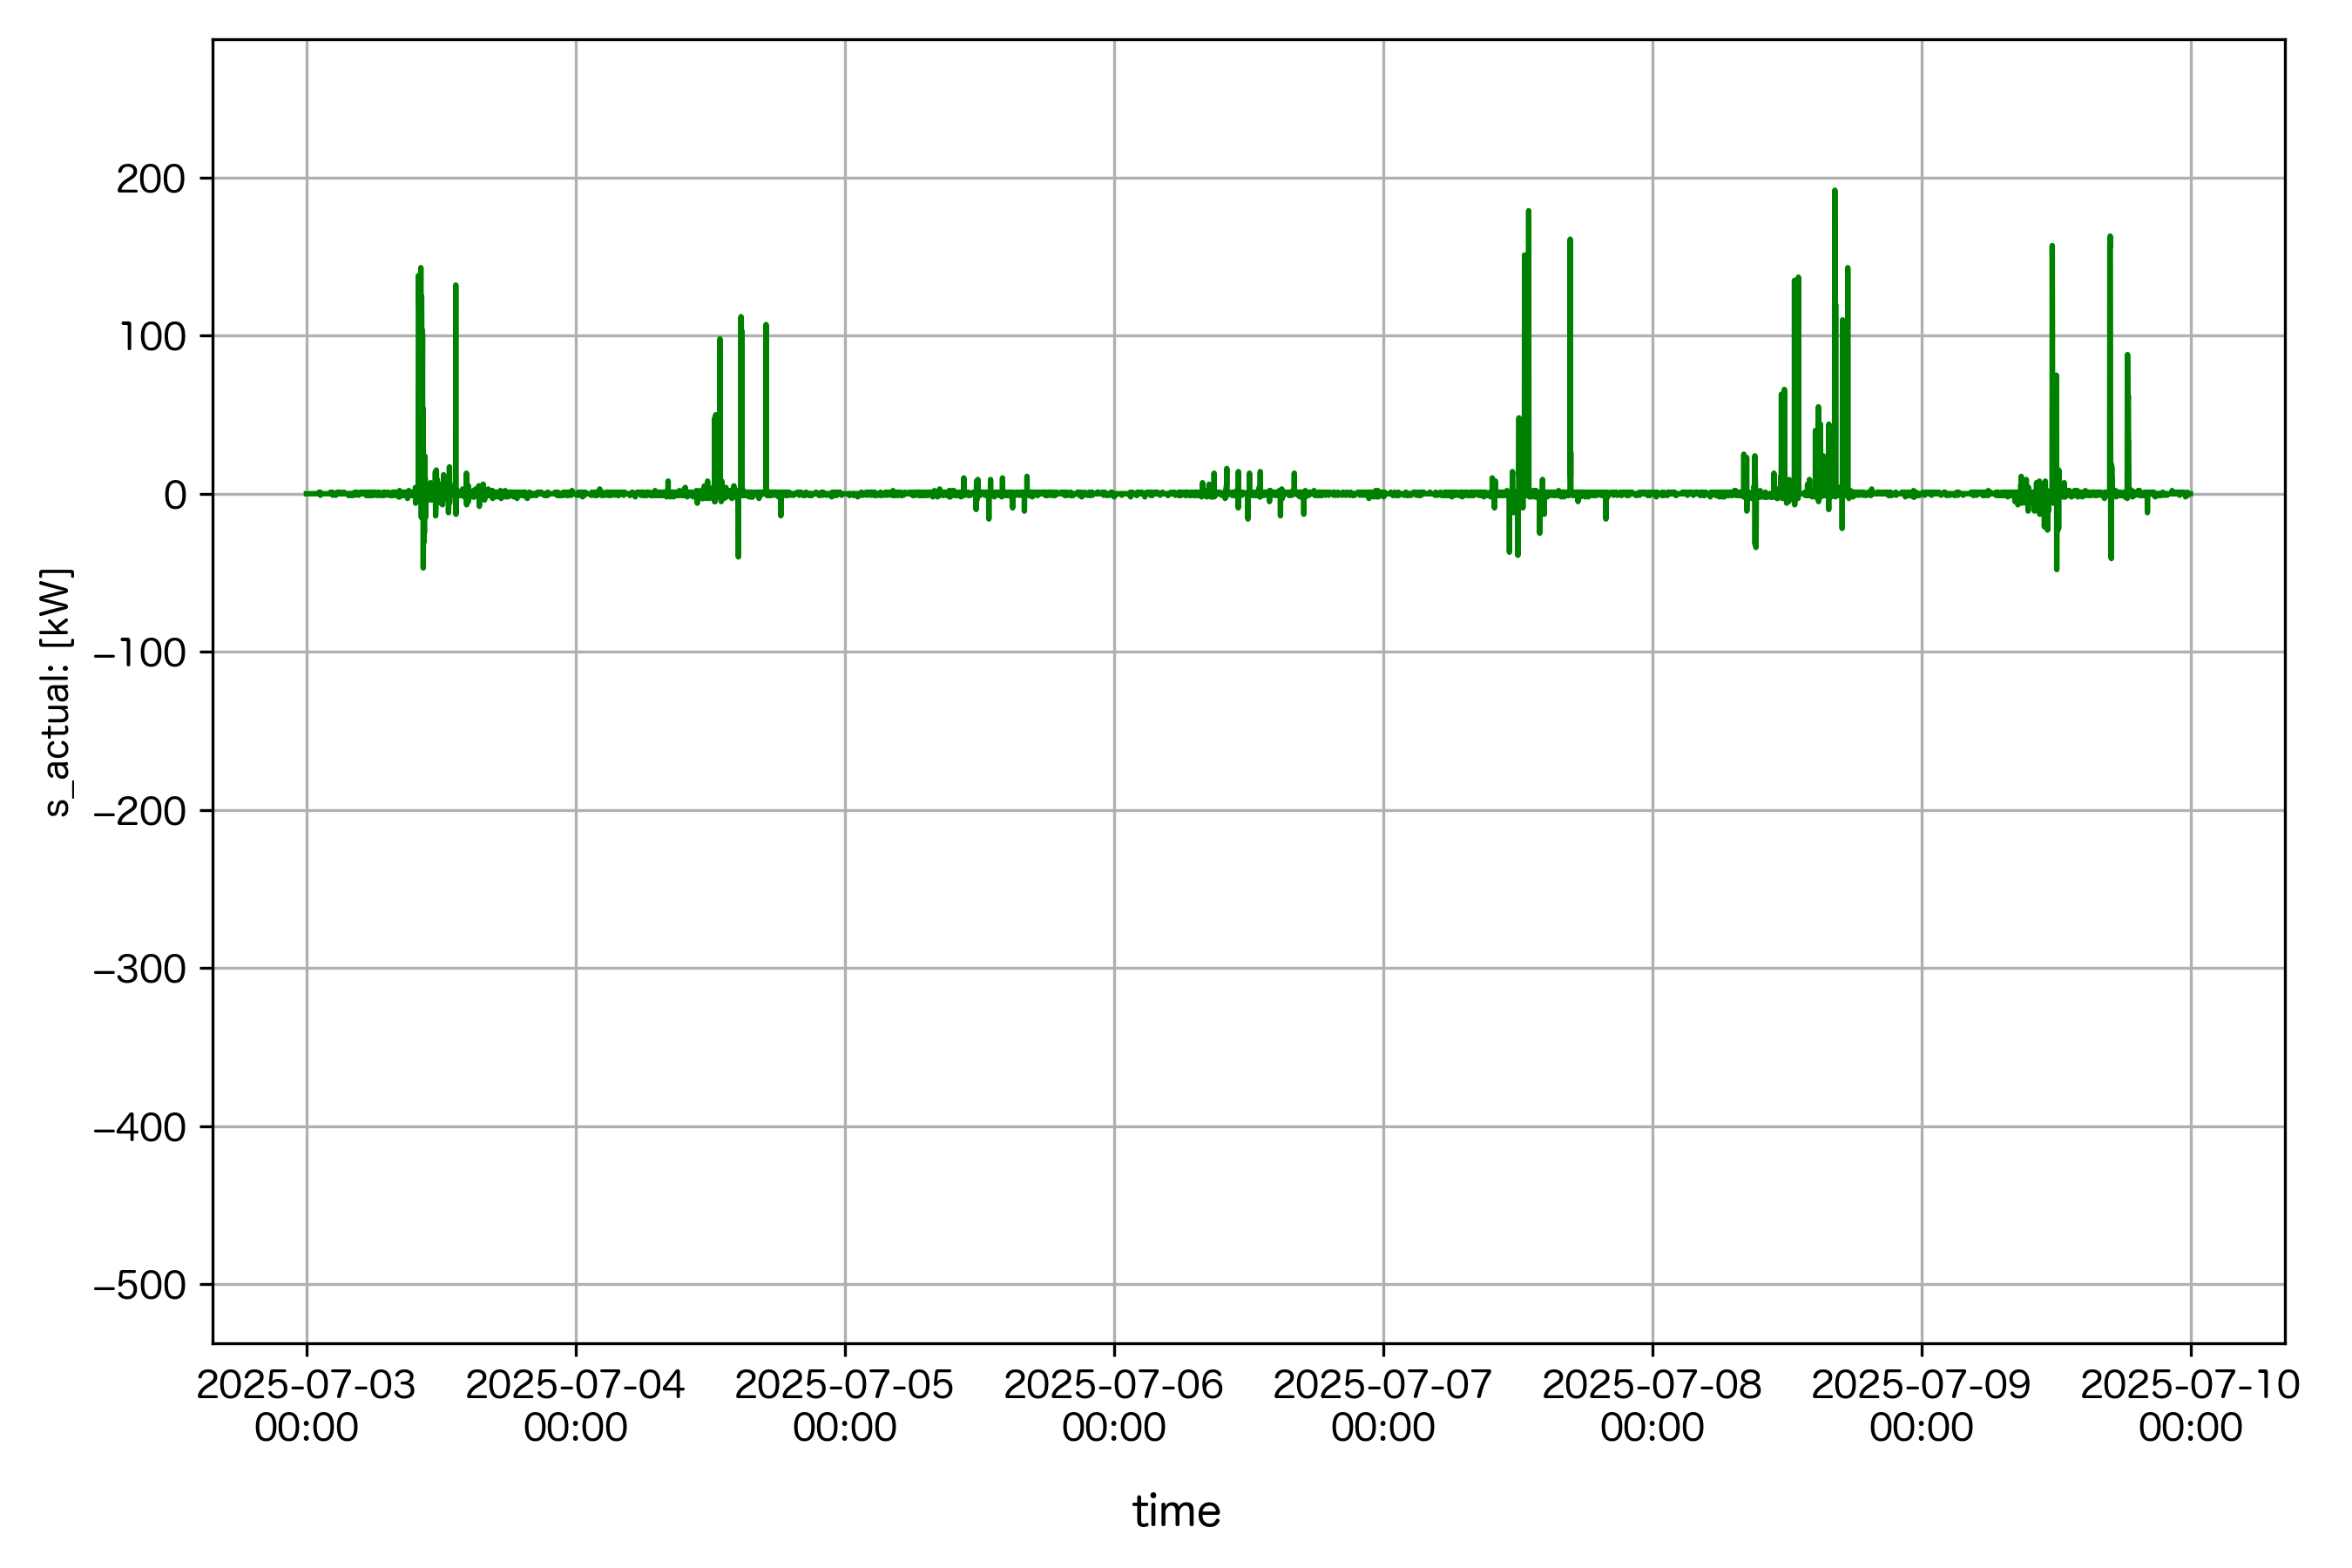
\includegraphics[width=\linewidth]{../png/s_actual.png}
      \end{minipage}
      \caption{系統買電の最適化結果と実績値の比較}
      \label{fig:s_compare}
\end{figure}

\begin{figure}[h]
      \centering
      \begin{minipage}[b]{\linewidth}
        \centering
        
\includegraphics[width=\linewidth]{../png/xFD1_xFC2.png} 
      \end{minipage}
      \hfill
      \begin{minipage}[b]{\linewidth}
        \centering
        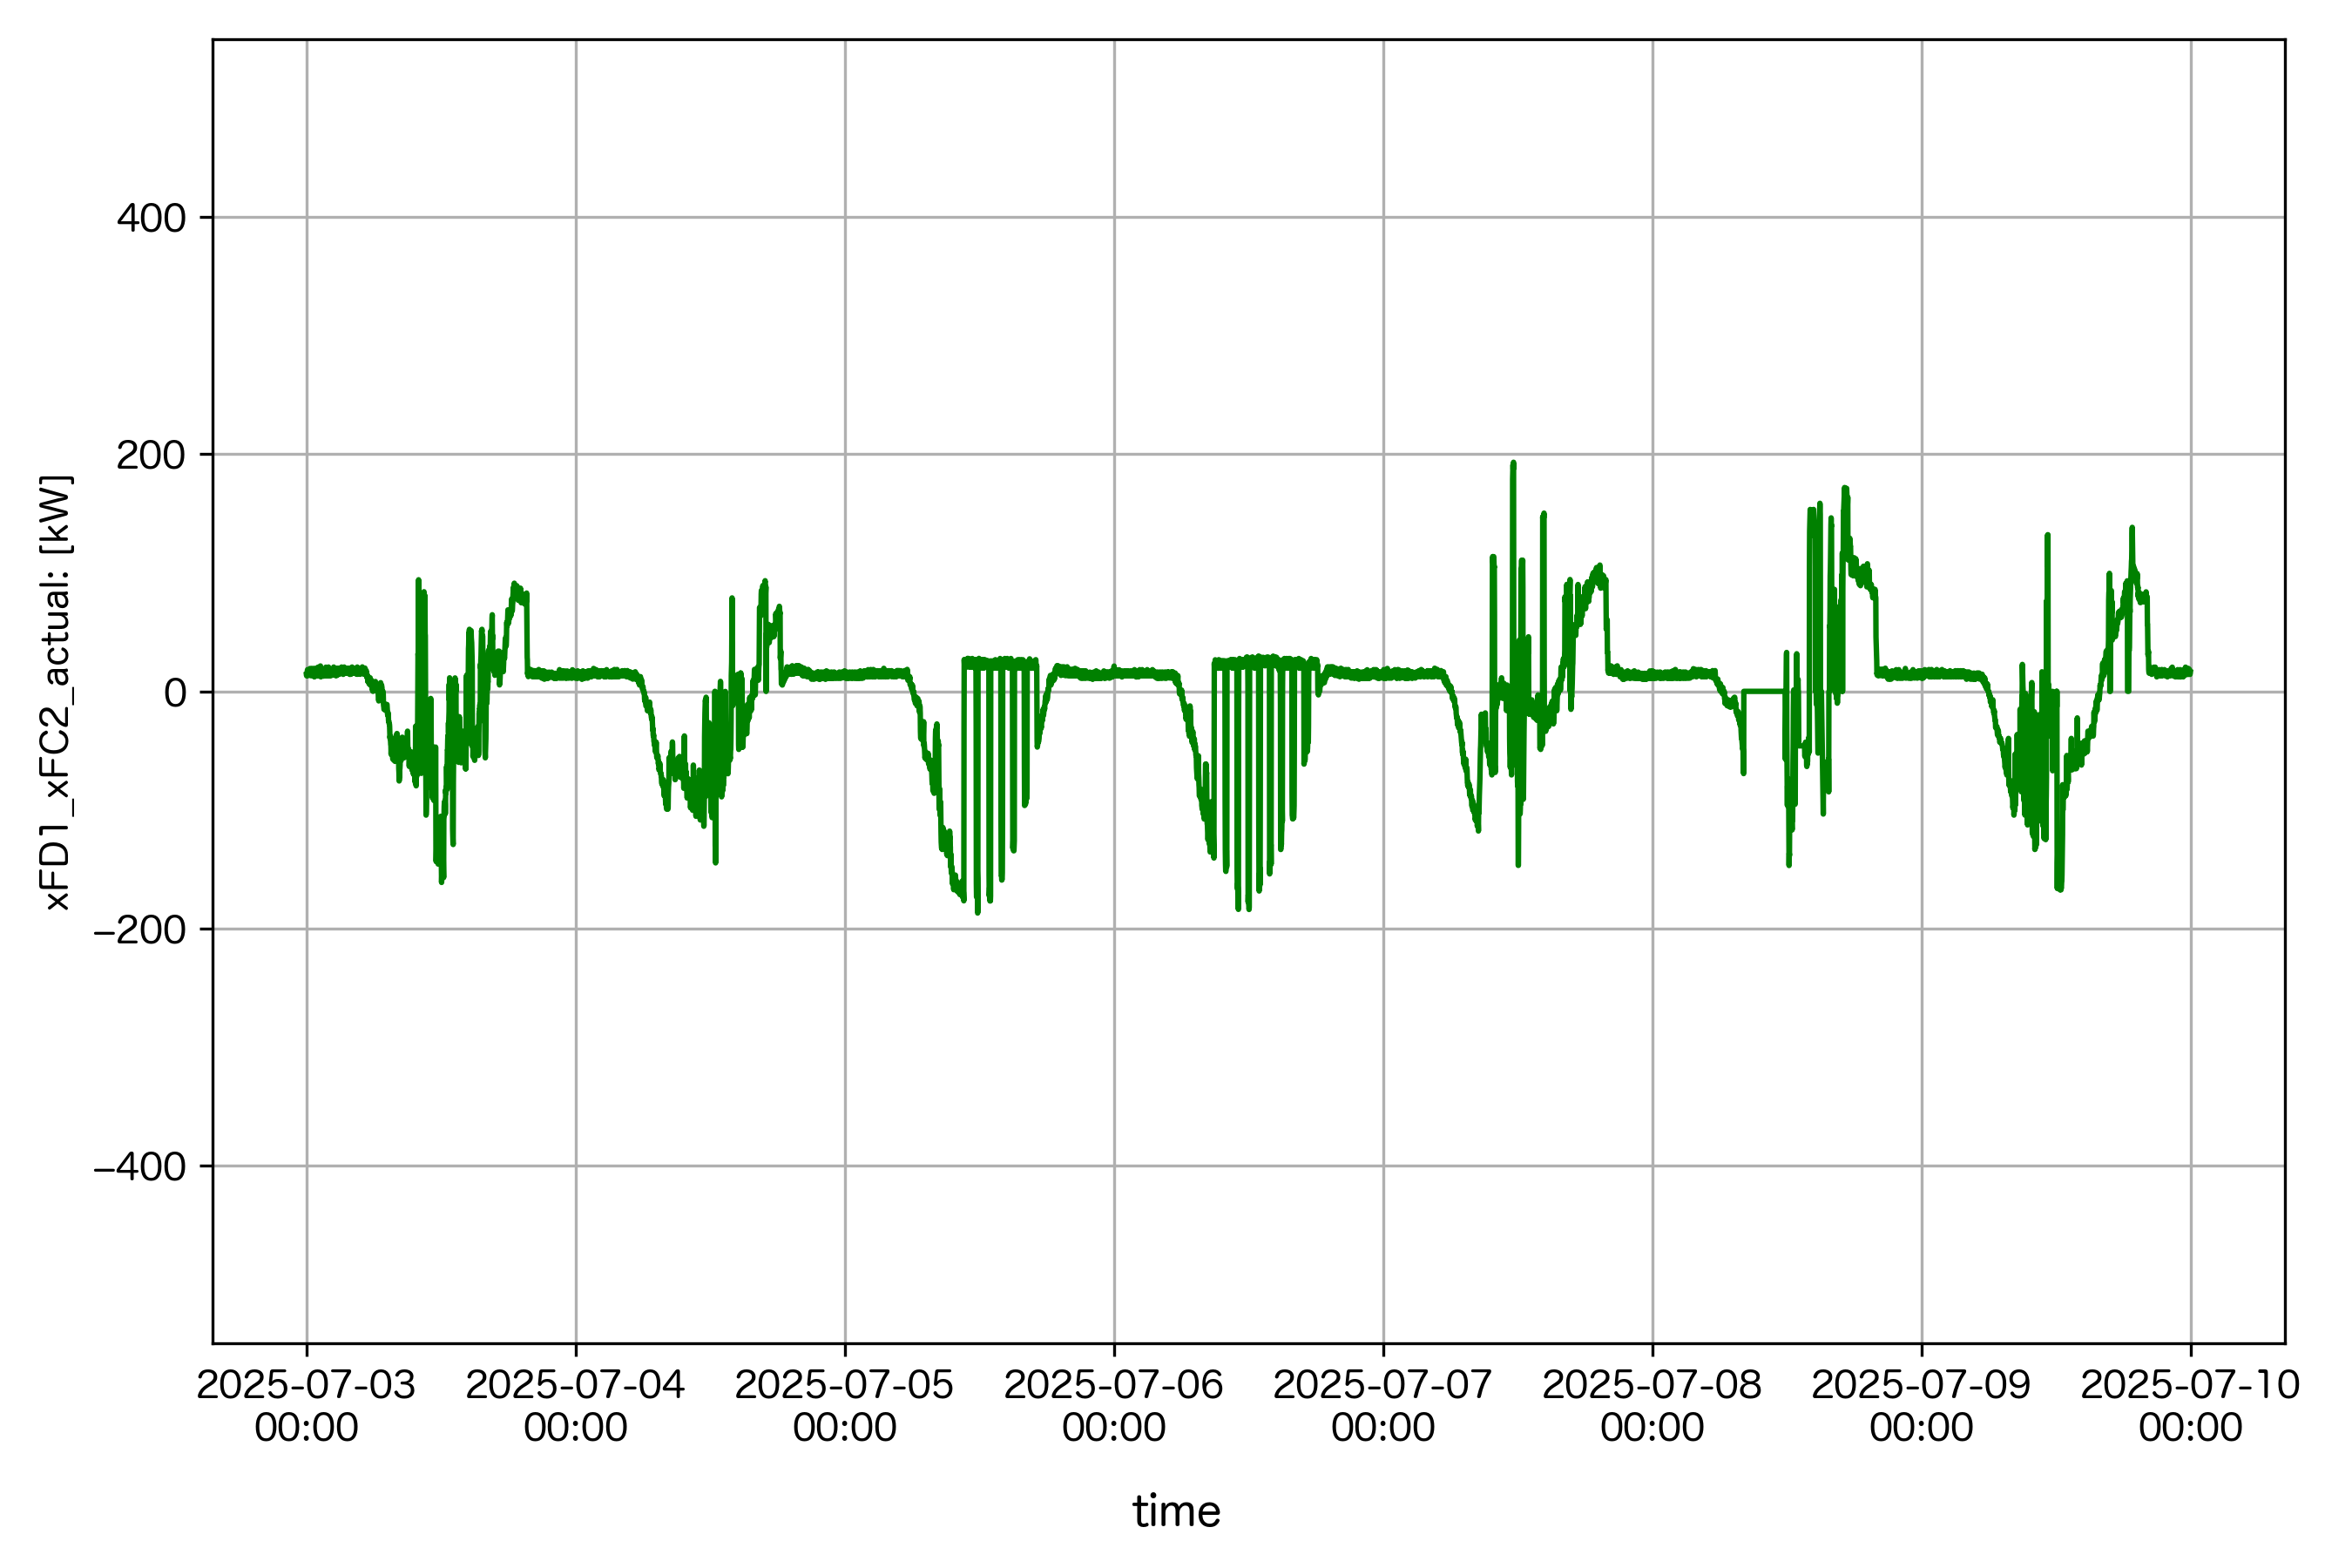
\includegraphics[width=\linewidth]{../png/xFD1_xFC2_actual.png}
      \end{minipage}
      \caption{バッテリー入出力の最適化結果と実績値の比較}
      \label{fig:x_compare}
\end{figure}

\begin{figure}[h]
      \centering
      \begin{minipage}[b]{\linewidth}
        \centering
        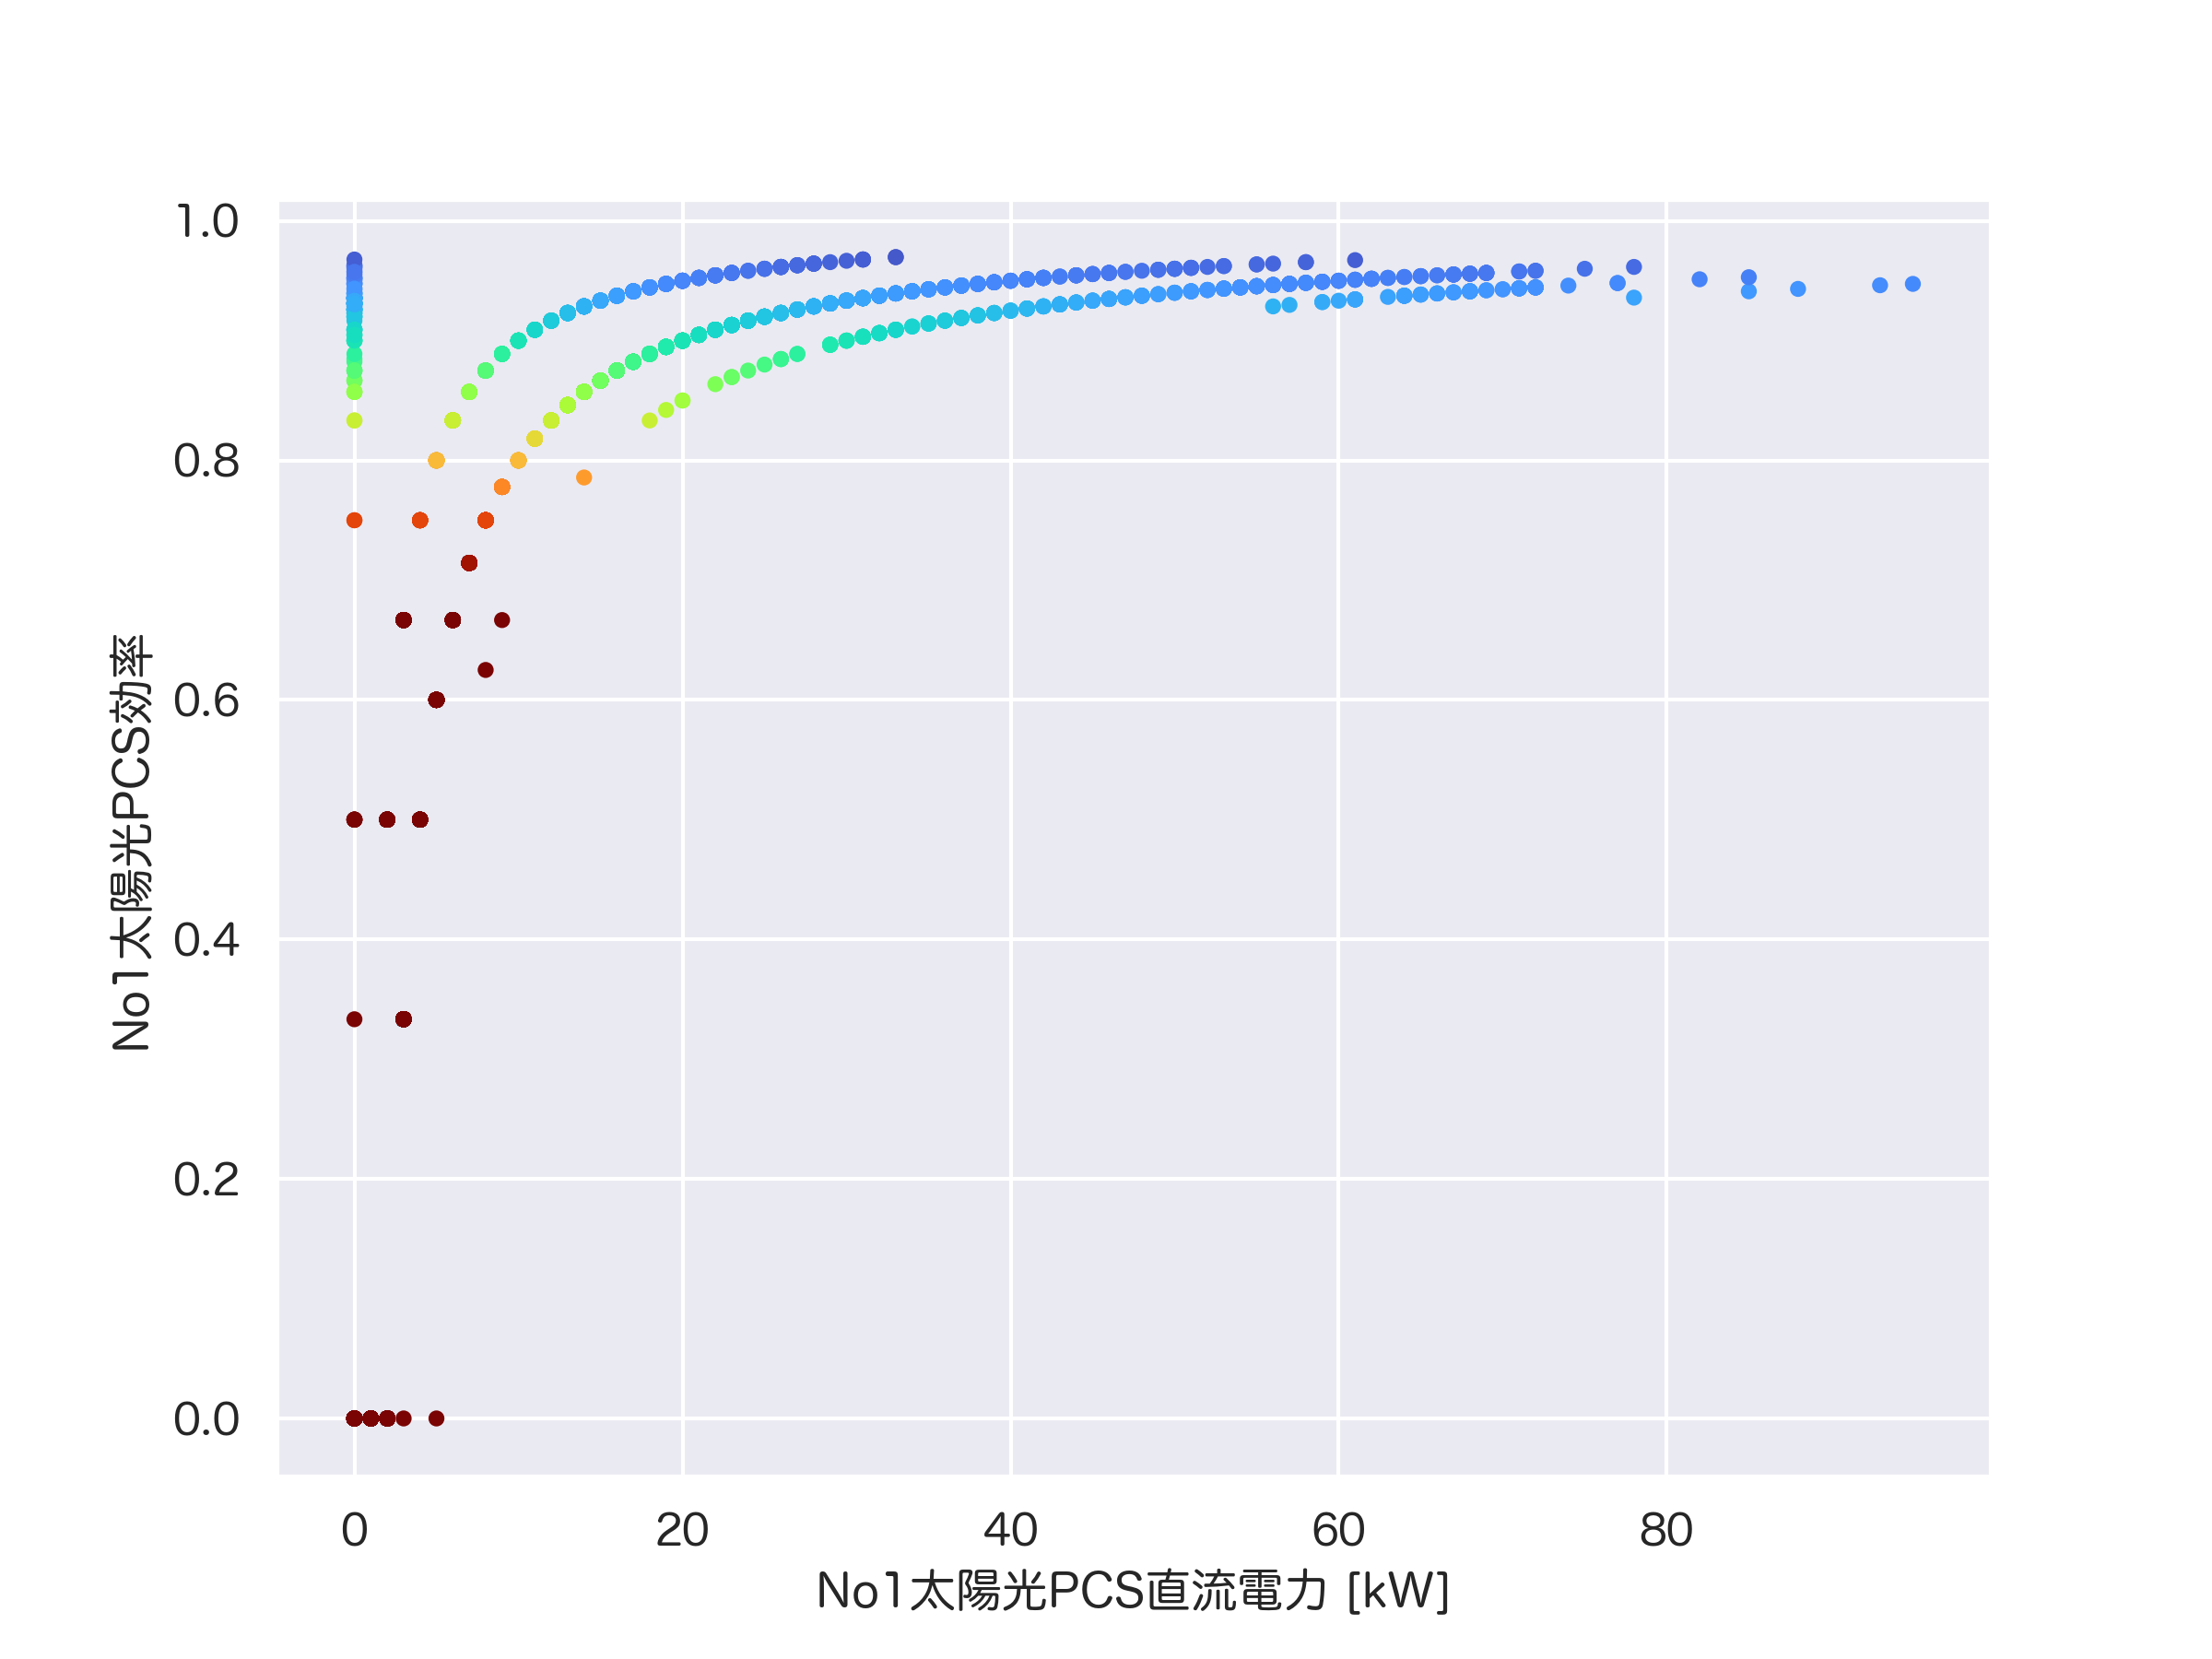
\includegraphics[width=\linewidth]{figure/efficiency-scatter.png} 
      \end{minipage}
      \hfill
      \begin{minipage}[b]{\linewidth}
        \centering
        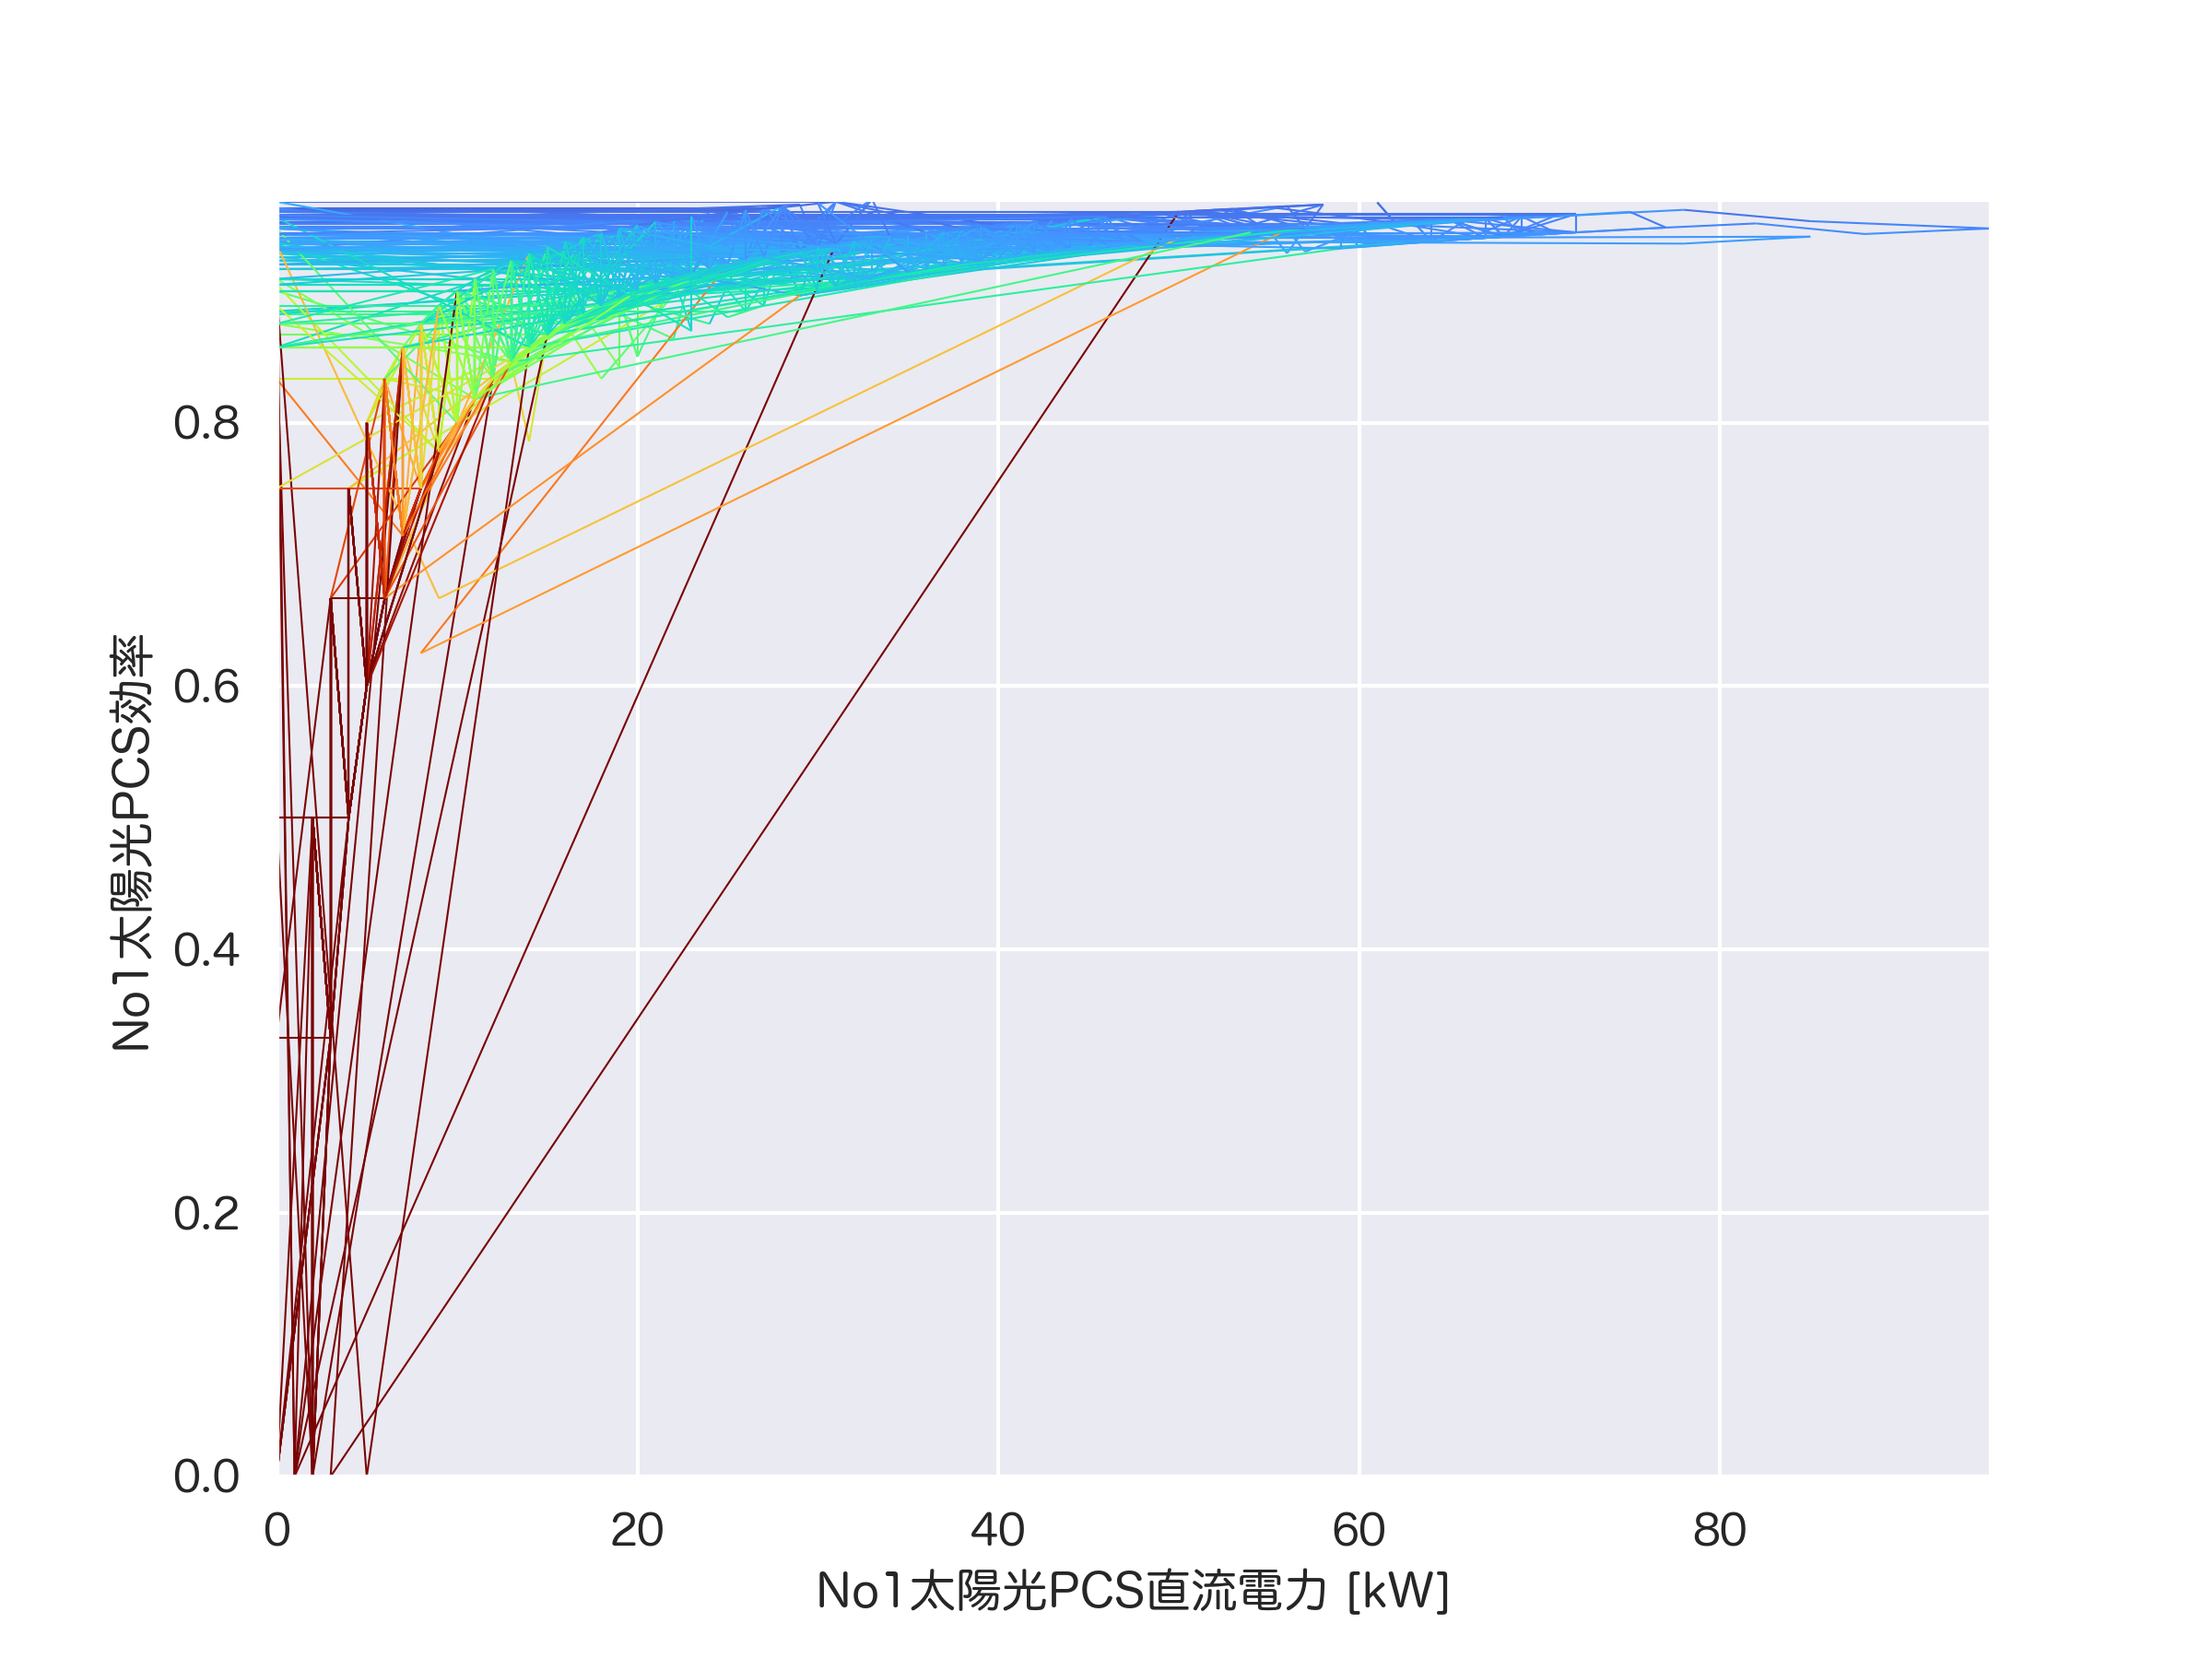
\includegraphics[width=\linewidth]{figure/efficiency-line.png}
      \end{minipage}
      \caption{PCSの入力電力と変換効率（下の図は，時間的に連続した点を線分で接続したもの）}
      \label{fig:PCS_efficiency1}
\end{figure}

\begin{figure}[h]
      \centering
      \begin{minipage}[b]{\linewidth}
        \centering
        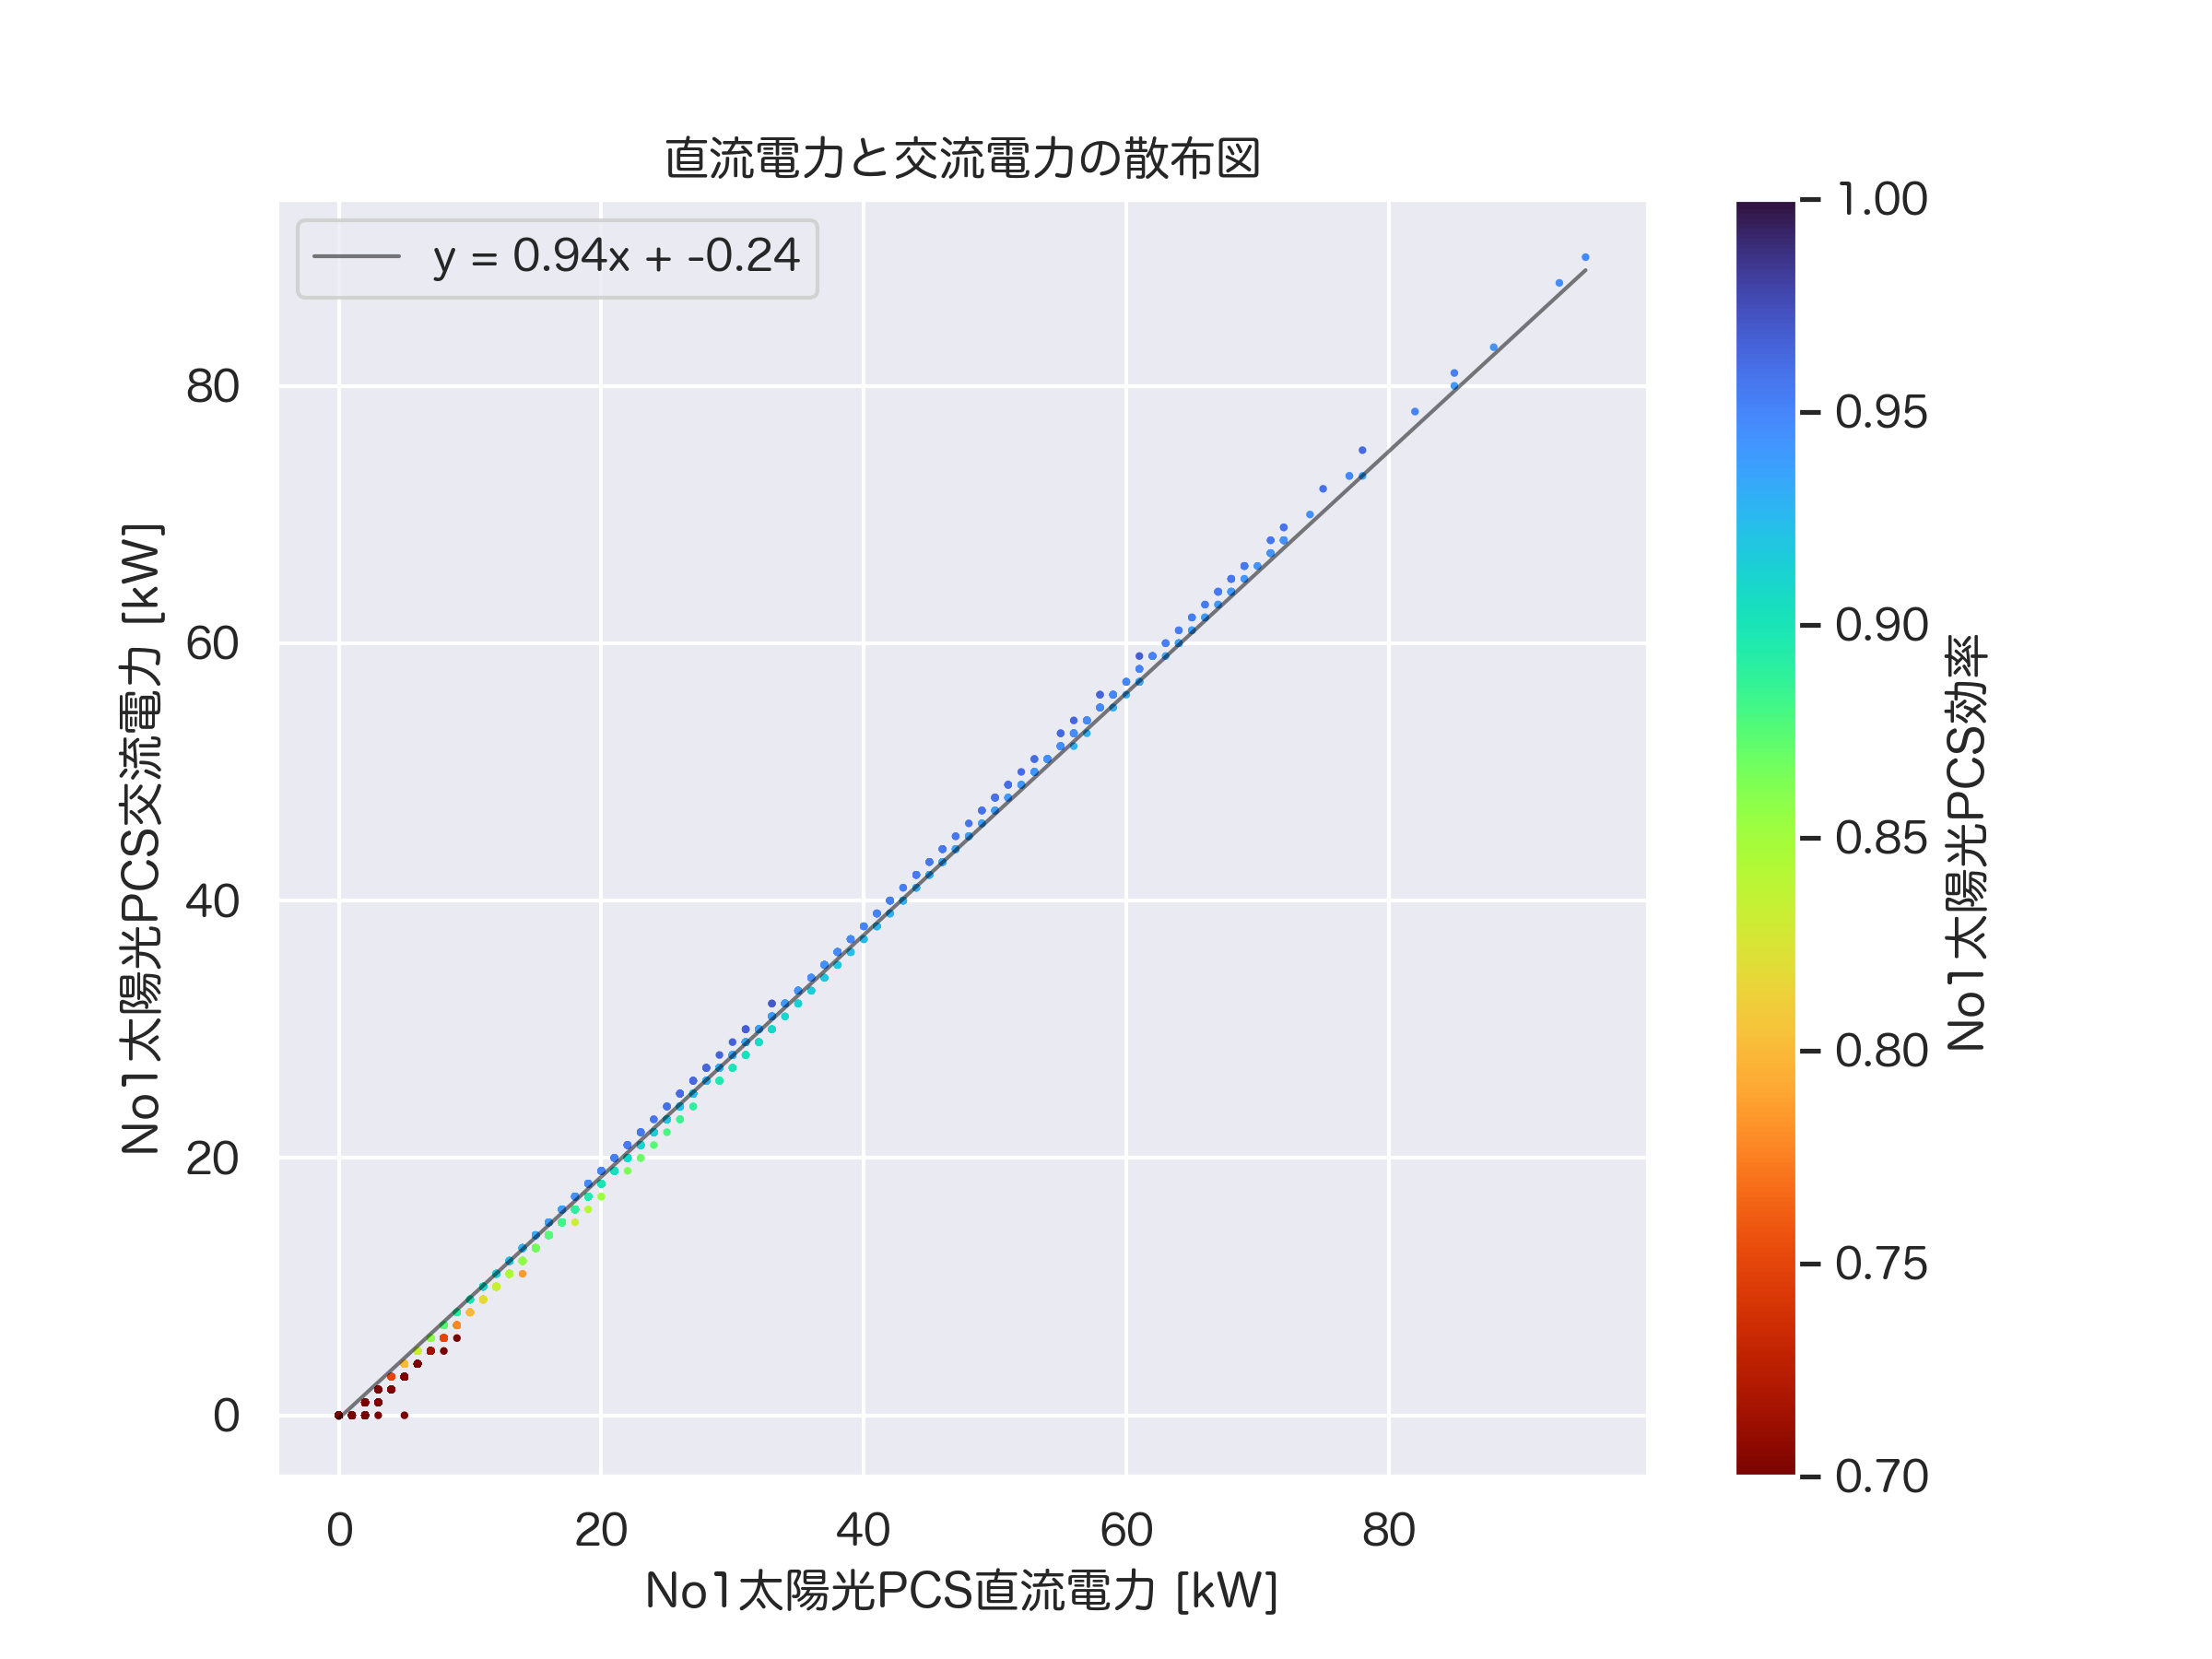
\includegraphics[width=\linewidth]{figure/PCS_IO1.png} 
      \end{minipage}
      \hfill
      \begin{minipage}[b]{\linewidth}
        \centering
        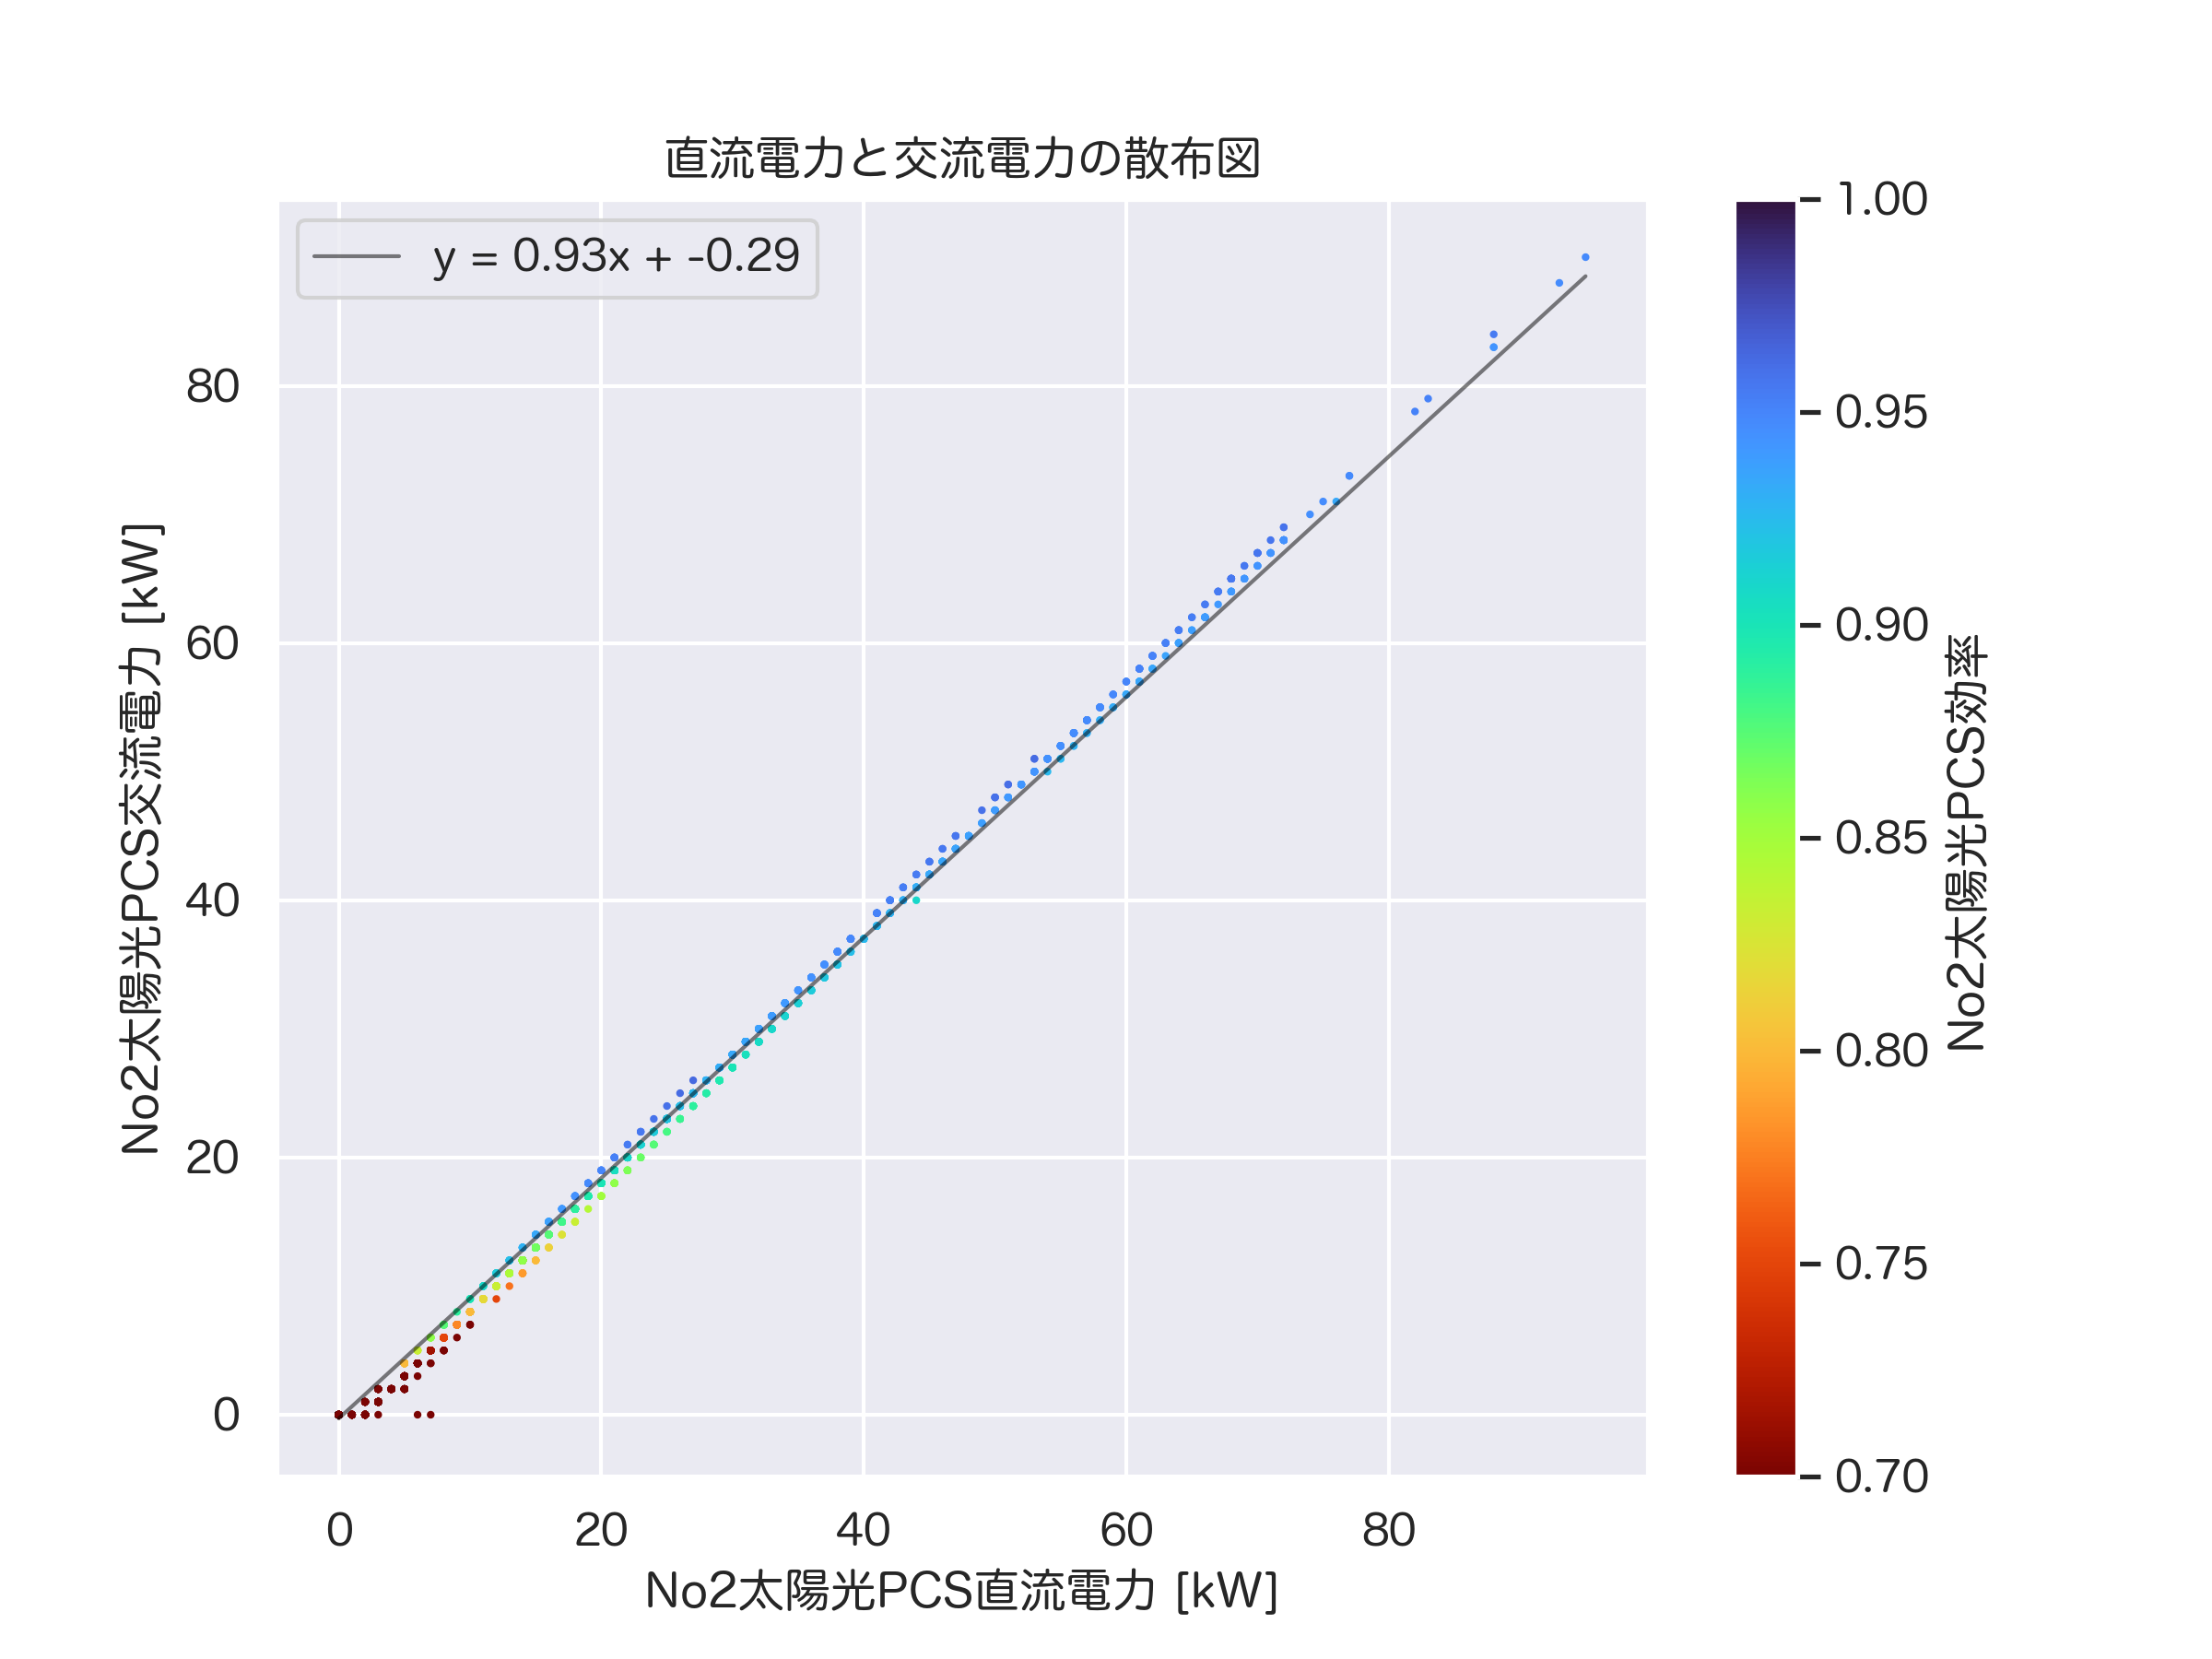
\includegraphics[width=\linewidth]{figure/PCS_IO2.png}
      \end{minipage}
      \caption{PCSの入力直流電力と出力交流電力}
      \label{fig:PCS_efficiency2}
\end{figure}

\clearpage

\end{document}
